\chapter{Gradi di libertà, struttura dei meccanismi e richiami}

	\section{Gradi di libertà}
		I \textbf{gradi di libertà} di un sistema meccanico sono pari al numero di variabili indipendenti che si devono specificare per descrivere il movimento.

		\vspace{0.5cm}
		\textbf{Esempi:}
			\begin{enumerate}

				\item La posizione di una particella posta su un piano può essere completamente definita:

					\begin{minipage}{.475\textwidth}
						\begin{itemize}
							\item una volta fissato un sistema di riferimento cartesiano, da due variabili indipendenti ($x_p$,$ y_p$)
							\item una volta assegnato l'angolo e il raggio (coordinate polari del punto), da due variabili indipendenti ($\rho$, $\alpha$)
						\end{itemize}
		
						Per definire la posizione di un punto sono sufficienti due variabili, di conseguenza si dice che la particella nel piano ha due gradi di libertà.
					\end{minipage}
					\hfill
					\begin{minipage}{.475\textwidth}
						\centering
						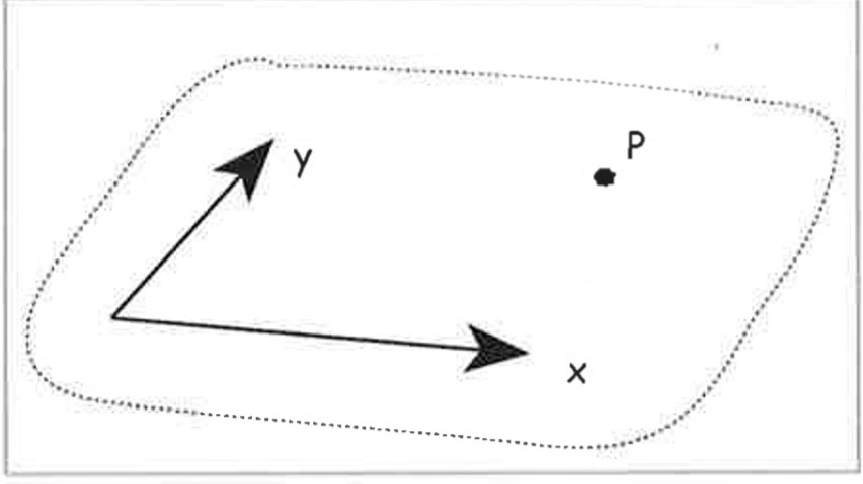
\includegraphics[width=.8\textwidth]{chapter02/immagine01} 
					\end{minipage}

				\vspace{3mm}
				\item Un corpo rigido nel piano ha invece tre gradi di libertà (una volta fissato un sistema di riferimento cartesiano):
				
					\begin{minipage}{.475\textwidth}
						\begin{itemize}
							\item due gradi di libertà possono essere associati alle coordinate di un punto qualsiasi di questo corpo rigido (posizione)
							\item il terzo all'angolo $\alpha$ dell'asse di simmetria con uno dei versori di riferimento (orientamento)
						\end{itemize}

					È possibile definire altri metodi per descrivere la posizione del corpo rigido nel piano, ma alla fine dobbiamo specificare sempre 3 variabili
					\end{minipage}
					\hfill
					\begin{minipage}{.475\textwidth}
						\centering
						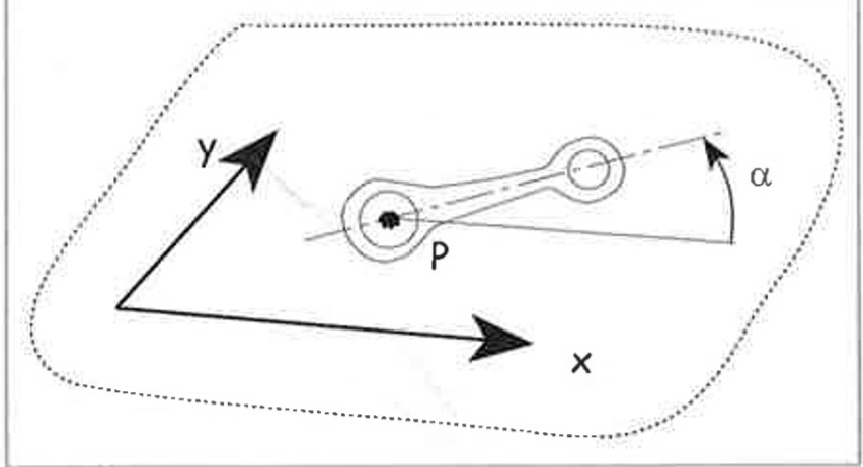
\includegraphics[width=.8\textwidth]{chapter02/immagine02} 
					\end{minipage}

				\vspace{3mm}
				\item Una particella libera di muoversi nello spazio ha 3 gradi di libertà: infatti sono necessarie solo 3 coordinate (cartesiane o sferiche) per descrivere completamente la sua posizione nello spazio.
				\item Un corpo rigido nello spazio ha 6 gradi di libertà, perché per descriverlo completamente sono necessarie:
	
					\begin{minipage}{.475\textwidth}
						\begin{itemize}
							\item 3 coordinate per specificare la posizione di un punto del corpo rigido nello spazio 
							\item 3  angoli per definirne l'orientamento
						\end{itemize}
					\end{minipage}
					\hfill
					\begin{minipage}{.475\textwidth}
						\centering
						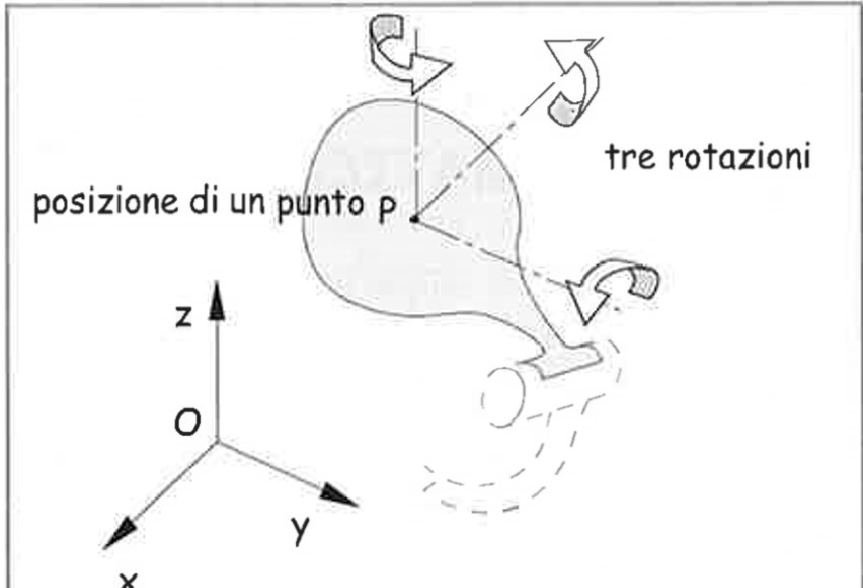
\includegraphics[width=.8\textwidth]{chapter02/immagine03} 
					\end{minipage}
			\end{enumerate}

		\vspace{1cm}
		Dagli esempi proposti si può dedurre facilmente che esistono diversi modi di associare i gradi di libertà alle varie coordinate, ma devono essere rispettati due requisiti:
			\begin{enumerate}
				\item Le coordinate devono essere {\scshape{\bfseries sufficienti}} a descrivere completamente il sistema
				\item Le coordinate devono essere {\scshape{\bfseries indipendenti }}
			\end{enumerate}

		Un insieme di coordinate sufficienti e indipendenti viene chiamato insieme di "coordinate generalizzate"

		\vspace{0.5cm}
		!! Il numero di gradi di libertà può essere diminuito imponendo dei vincoli al corpo o al sistema di corpi rigidi in esame.
		In tal caso si parla di {\scshape{\bfseries equazione di vincolo di corpo rigido }}(=corpo non deformabile). \newline

		\textbf{Esempio:} nell'occasione della definizione della posizione di un corpo sono sufficienti le coordinate del punto P $(x_p, y_p)$  e l'angolo $\alpha$ a descrivere il sistema, infatti se sono asssegnate il corpo rigido può avere una sola posizione e un solo orientamento. (Figura a sinistra)

		Alternativamente se avessimo preso le coordinate di due punti su un piano non avrei avuto bisogno di tutte e 4 le variabili ($x_a, x_b, y_a, y_b$) [con A e B due punti materiale del corpo in questione]
		bensì solo di 3 in quanto il corpo, essendo rigido e dunque indeformabile, impone un'equazione di vincolo fisso sulla distanza dei punti A e B. (figura a destra)

			\begin{figure}[h]
				\centering
				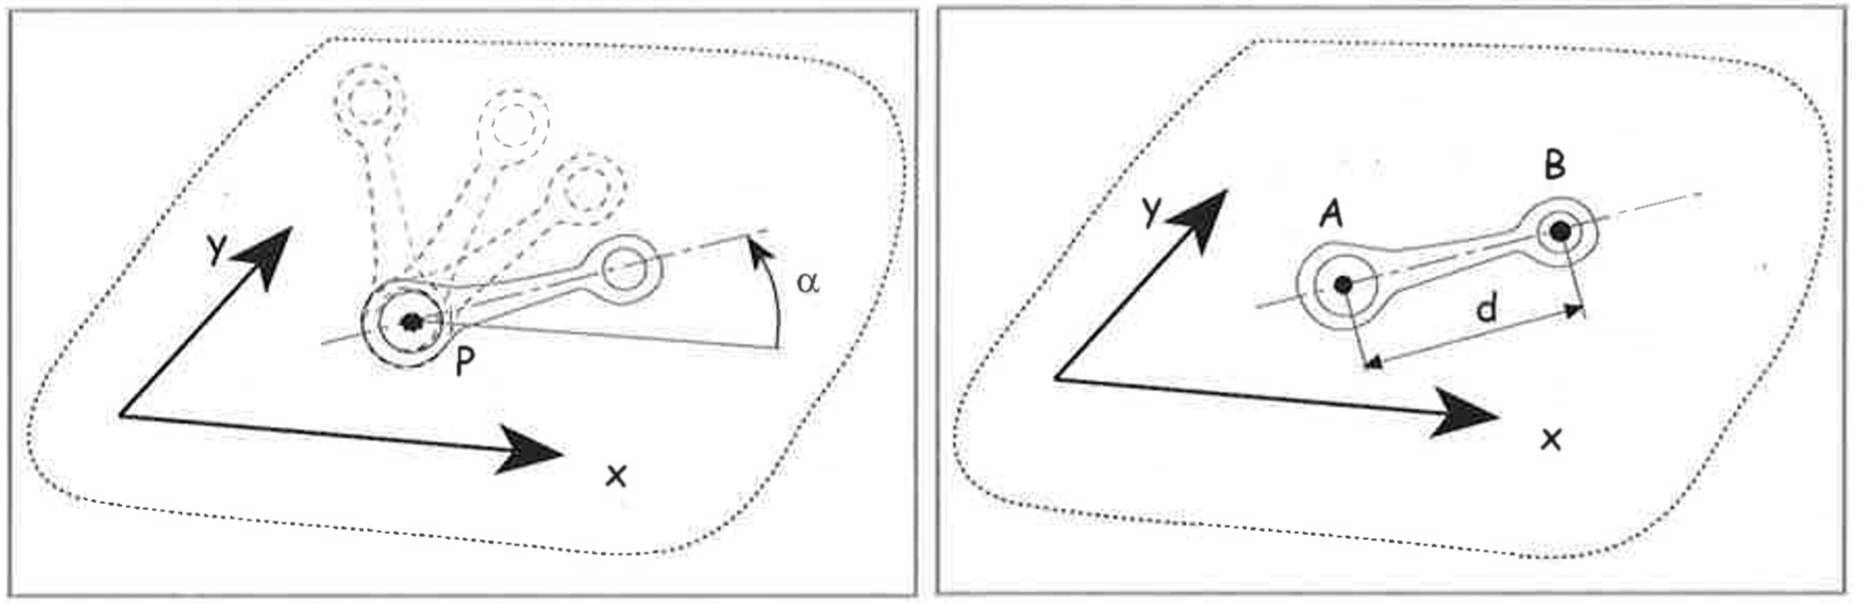
\includegraphics[width = 0.6\textwidth]{chapter02/immagine04}
			\end{figure}
			\begin{center}
				I punti in questione, infatti, sono vincolati a tenersi alla medesima distanza:
			\end{center}
			\begin{equation*}
				d = \sqrt{(x_a - x_b)^2 + (y_a - y_b)^2} = cost
			\end{equation*}
			Si può notare che imponendo tale vincolo una delle variabili scelte risulta essere rindondante e può essere ricavata dall'equazione di vincolo conoscendo le 3 rimanenti.

	\section{Coppie cinematiche piane}

		I corpi rigidi interagiscono tra loro all'interno di uno stesso sistema meccanico per via di collegamenti reciproci che ne limitano i gradi di libertà.
		Tali limiti imposti sul moto relativo fra i corpi sono chiamati {\scshape{\bfseries vincoli}}.\newline

			** \textbf{Elementi cinematici} := superfici dei due corpi fra loro a contatto della coppia.

			** \textbf{Coppia cinematica}\hspace{2mm} := sistema che accoppia due membri e che quindi toglie alcuni gradi di libertà del moto relativo 
	   
		Nel piano possiamo distinguere tra 3 coppie cinematiche:
\newpage

		\begin{enumerate}
			\item \textbf{Coppia rotoidale (R)} o \textbf{Cerniera}

				\begin{minipage}{.6\textwidth}	
					Consideriamo due corpi rigidi nel piano. Ognuno di essi prevede 3 gradi di libertà che identificano la posizione di un loro punto materiale nel piano
					e uno che ne identifica l'orientamento (es. angolo rispetto all'orizzontale).\newline
					La \textbf{coppia rotoidale} o \textbf{cerniera} consiste nell'accoppiamento di una superficie cilindrica piena (appartenente ad un corpo) e di una superficie cilindrica vuota (appartenende all'altro corpo)
					con medesimo raggio (per ovviare al problema della presenza di giochi tra i due componenti; questo tipo di coppia priva di giochi è anche chiamata {\scshape{\bfseries combaciante}}).
					
					Se i raggi sono idealmente uguali un corpo sarebbe capace di ruotare intorno al centro della cerniera il che equivale a dire che i 2 corpi condividono/hanno 2 punti coincidenti
				\end{minipage}
				\hfill
				\begin{minipage}{0.3\textwidth}
					\centering
					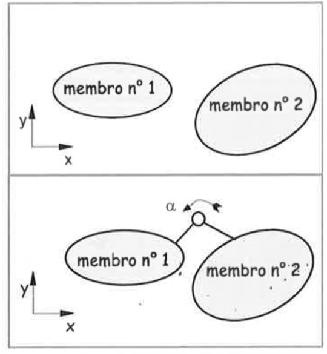
\includegraphics[width = \textwidth]{chapter02/immagine05}
				\end{minipage}

				\begin{itemize}
					\item per cui le equazioni di congruenza che rappresentano/descrivono questa coppia cinematica saranno:
						\begin{equation*}
							x(p_1) = x(p_2) \hspace{1.5cm}  y(p_1) = y(p_2)
						\end{equation*}
					\item tale vincolo è dovuto all'accoppiamento dei due corpi e alla rotazione relativa di uno rispetto all'altro attorno al punto in cui è presente la cerniera
				\end{itemize}

			\begin{figure}[h]
				\centering
				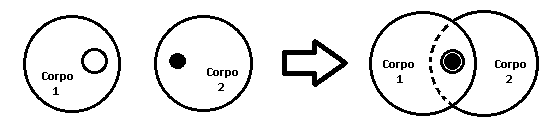
\includegraphics[width = 0.8\textwidth]{chapter02/immagine06}
			\end{figure}

						In conclusione: due corpi separati hanno 3 gradi di libertà ciascuno;
						due corpi incernierati hanno 2 varibili rindondanti (ovvero, combinati, 4 gradi di libertà)

					\item \textbf{Coppia prismatica (P)}

						Nel caso si voglia che sopravviva un moto relativo di traslazione è possibile decidere di applicare una coppia prismatica: essa consiste nella realizzazione di una cava rettangolare su un corpo e di un prisma sull'altro corpo (idealmente le superfici devono essere: uguali, in modo da permetterne lo scorrimento, e avere le stesse dimensioni).

			\begin{figure}[h]
				\centering
				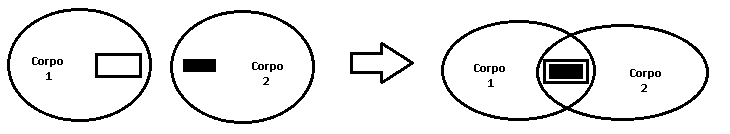
\includegraphics[width = .75\textwidth]{chapter02/immagine07}
			\end{figure}

				Al fine di rappresentare la coppia prismatica devo definire in primo luogo l'asse (identificato dai vettori $\mathbf{u_1}$ e $\mathbf{u_2}$) e la posizione dell'elemento prismatico ($p_1$, $p_2$) in questione.

			\begin{minipage}{.45\textwidth}
				A partire da tali dati sui due corpi devo successivamente imporre i seguenti vincoli:
				\begin{enumerate}
					\item u1 e u2 devono essere paralleli, ovvero il prodotto vettoriale/esterno dei vettori degli assi deve essere nullo
						(in questo modo l'angolo di rotazione di entrambi i corpi sarà lo stesso)
						\[ \mathbf{u_1} \wedge \mathbf{u_2} = 0\]
					\item la distanza di $p_2$ dal vettore $\mathbf{u_1}$ deve essere nulla  \[d_{p_2 \to u_1} = 0\]
				\end{enumerate}
			\end{minipage}
			\hfill
			\begin{minipage}{.45\textwidth}
				\centering
				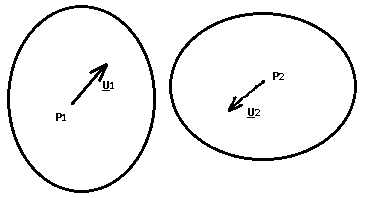
\includegraphics[width = \textwidth]{chapter02/immagine08}
			\end{minipage}

			In questo modo rimane libera la traslazione nella direzione dell'asse comune ai 2 elementi prismatici

			\textbf{OSS}: \begin{itemize} \item le precedenti coppie cinematiche hanno superfici cinematiche coincidenti/presentano contatto superficiale
								\item La seguenti rappresentazioni, assieme a quelle già proposte precedentemente, della coppia prismatica sono ammesse:

				\begin{figure}[h]
					\centering
					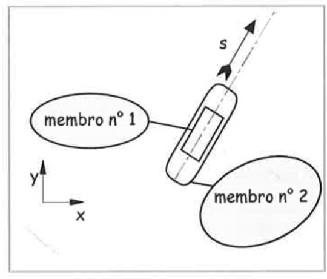
\includegraphics[width =0.3\textwidth]{chapter02/immagine09}
					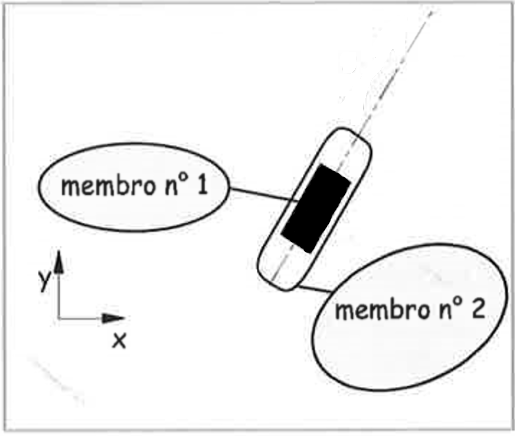
\includegraphics[width =0.3\textwidth]{chapter02/immagine10}
					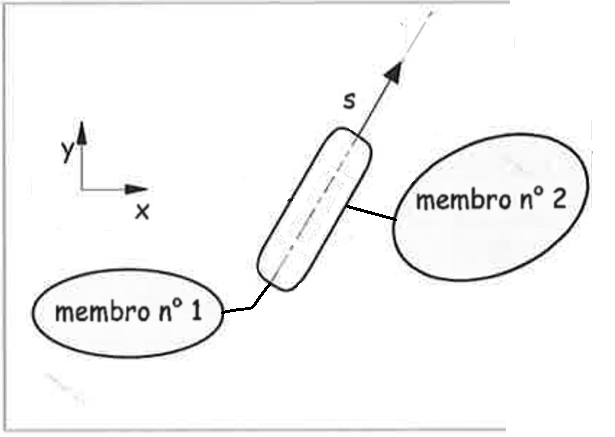
\includegraphics[width =0.4\textwidth]{chapter02/immagine11}
				\end{figure}

			\end{itemize}

			\item \textbf{Coppia a camma (C)}
	
				Contrariamente alle precedenti coppie cinematiche in cui venivano eliminati 2 gradi di libertà, la coppia a camma permette di eliminare solo un grado di libertà (ovvero la traslazione lungo una direzione). 

				\begin{minipage}{.25\textwidth}
					\centering
					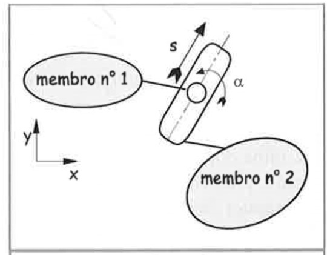
\includegraphics[width = \textwidth]{chapter02/immagine12}
				\end{minipage}
				\hfill	
				\begin{minipage}{.7\textwidth}
					Essa viene schematizzata da:
	\begin{itemize}
	\item Una guida prismatica connessa al corpo 1 
	\item Un cilindro di diametro pari alla dimensione della cava/guida connessa al corpo 2
\end{itemize}
\end{minipage}
\vspace{2mm}

	In tal modo il cilindro può scorrere all'interno della cava e ruotare su se stesso.

\begin{minipage}{.45\textwidth}
Il vincolo da imporre in tale situazione è che il punto $p_2$ (ovvero il centro/asse del cilindro) sia sull'asse della cava e viene rappresentata dall'equazione di vincolo  \[(p_1,p_2) \parallel \mathbf{u_1}\]
Ovvero che il vettore che collega i due punti in questione sia parallelo all'orientazione della cava prismatica che farà da guida al cilindro.
\end{minipage}
\hfill
\begin{minipage}{.45\textwidth}
\centering
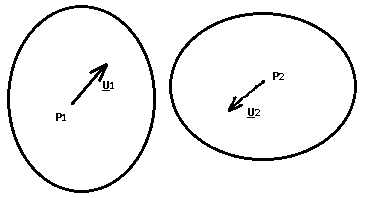
\includegraphics[width = .8\textwidth]{chapter02/immagine08}
\end{minipage}
\end{enumerate}


\vspace{2mm}
\textbf{OSS}: \begin{itemize}
\item Nella coppia a camma si ha contatto su una dimensione/un punto nel piano non sulla linea o tutte le superfici, come invece avveniva per la coppia rotoidale e la coppia prismatica (\emph{contatto non combaciante})	
\item a volte la realizzazione di tale coppia impiega mezza cava prismatica (in questa situazione la coppia si definisce \textbf{unilaterale} e il vincolo è anch'esso definito unilaterale)

\begin{minipage}{.65\textwidth}
	\begin{itemize}
		\item il vincolo bilaterale (descritto precedentemente) prende, dunque, un accoppiamento di forma (chiusa) o a comando positivo [la forma stessa degli elementi cinematici è sufficiente a mantenere il contatto]
		\item il vincolo unilaterale prende, invece, un accoppamento di forza o di forma aperta [per mantenere la coppia è necessaria una forza]
			(cfr. comando desmodromico)
	\end{itemize}
	\end{minipage}
	\hfill
	\begin{minipage}{.35\textwidth}
	\centering
	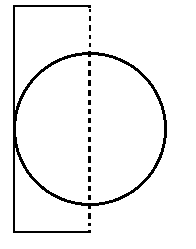
\includegraphics[width = .5\textwidth]{chapter02/immagine13}
	\end{minipage}

\item Non si è vincolati ad avere l'asse della camma rettilinea (essa può assumere qualsiasi forma), per questa ragione è necessario introdurre il concetto di:

{\scshape{\bfseries Profili coniugati}} := profili di due corpi che vengono a contatto durante il moto dove non è presente un vera e propria coppia a camma, ma tale coppia è realizzata dalla opportuna profilazione dei due corpi coinvolti

\begin{figure}[h]
\centering
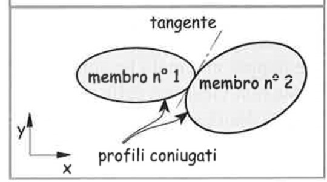
\includegraphics[width = .3\textwidth]{chapter02/immagine14}
 \end{figure}
 

 
\item Nelle concrete realizzazioni, gli elementi cinematici possono essere rigidi o deformabili
\begin{itemize} \item Gli elementi cinematici si possono accoppiare tra di loro in modo tale da realizzare un contatto su superficie estesa (combaciante)
		\item oppure un contatto lineare o puntiforme (tipico della coppia a camma) (non combaciante)
\end{itemize}
\item Le coppie cinematiche realizzate con elementi rigidi e combacianti che lasciano un solo grado di libertà relativo sono dette coppie elementari od inferiori
		(aka rotoidale e prismatica)
\item Le altre coppie cinematiche sono chiamate superiori e sono realizzate con membri rigidi aventi elementi cinematici non combacianti oppure membri rigidi aventi elementi cinematici combacianti 
		(aka cinghie che sono corpi non estensibili ma flessibili).
		
		Delle coppie di classe superiore si distinguono, difatti, diverse classi in base al numero di gradi di libertà che lasciano liberi (ossia non vincolati dalla coppia)
 \end{itemize}

 Il contatto tra gli elementi cinematici può essere:
 \begin{enumerate}
\item di puro rotolamento se la velocità nel punto di contatto è nulla ({\scshape{\bfseries senza strisciamento}})
\item di strisciamento se la velocità tra le superfici a contatto non è nulla ({\scshape{\bfseries con strisciamento}}) [$\Rightarrow$ favorisce l'usura del pezzo]
\item d'{\scshape{\bfseries urto}} se la velocità relativa dei due elementi cinematici ha una componente non nulla nella direzione normale alle superfici
	-> la realizzazione di giochi per l'accoppiamento è  particolarmente soggetto ad urti che ne determina un aumento dell'usura superficiale, vibrazione, e perdita di performance.
 \end{enumerate}

\section{Struttura dei meccanismi}

È giunto il momento di discutere su come mettere insieme un certo numero di corpi a formare un sistema/macchina\newline

{\scshape{\bfseries membro}} := elemento di una macchina in movimento rispetto agli altri e ad essi connesso tramite coppie cinematiche

\vspace{2mm}
\noindent Il membro che è fisso rispetto al riferimento assoluto è detto {\scshape{\bfseries telaio}} (corpo rispetto a cui vado a studiare il movimento / di riferimento)

\noindent Un membro che è connesso agli altri tramite due coppie cinematiche viene detto \emph{binario}\\
Un membro che è connesso agli altri tramite tre coppie cinematiche viene detto \emph{ternario}\newline


Tradizionalmente i diversi membri binari si distinguono in:
 \begin{itemize}
 \item \textbf{Manovelle}: se hanno  
 	\begin{itemize} \item due coppie rotoidali, di cui una fissa a telaio,
					\item possono ruotare di 360 $\si{deg}$ rispetto a telaio
		\end{itemize}
		\item \textbf{Bilanciere} : se hanno	
		\begin{itemize}\item due coppie rotoidali di cui una fissa a telaio 
					\item non riescono a compiere una rotazione completa rispetto al telaio
		\end{itemize}
		\item \textbf{Bielle}: se hanno due coppie rotoidali entrambe non a telaio
\end{itemize}

Un sistema di membri connessi tra di loro da coppie cinematiche formano una {\scshape{\bfseries catena cinematica}}.

Queste possono essere:
\begin{itemize}
\item \textbf{Chiuse} = se forma uno o più anelli chiusi
\item \textbf{Aperti} = se presenta uno o più rami aperti
\end{itemize}

La differenza concettuale tra catena cinematica e meccanismo risiede nel momento in cui viene scelto il telaio:
\begin{itemize}
\item una  \textbf{Catena cinematica} è un sistema/insieme di membri in cui non è stato ancora definito un telaio
\item un \textbf{Meccanismo} è un sistema/insieme di membri in cui è presente un telaio
\end{itemize}

Da tale definizione si può denotare che da una stessa catena cinematica possono essere definiti più meccanismi, in quanto ogni membro della catena può essere definito come telaio.
Procediamo, dunque, a osservare più nel dettaglio le possibili catene cinematiche che si possono estrapolare dalla diversa combinazione delle sue proprietà:\newline

La più semplice e comune catena cinematica chiusa è la catena a quadrilatero che è formata da quattro  membri binari.\newline
\noindent Nel caso in cui le quattro coppie cinematiche siano rotoidali da questa catena deriveranno tutti i meccanismi del tipo a quadrilatero articolato (vengono proposti degli esempi nella figura a lato, in cui dalla catena cinematica sono stati scelti come telaio, rispettivamente, il membro 3 e 4)


\begin{SCfigure}[][h]
\centering
\caption*{
\textbf{Figura a sinistra}: \newline
Membro 1 e 3 bilanciere;\newline
Membro 2 biella;\newline
Membro 4 telaio.\newline

\textbf{Figura a destra}: \newline
Membro 2 e 4 bilanciere;\newline
Membro 1 biella;\newline
Membro 3 telaio.}
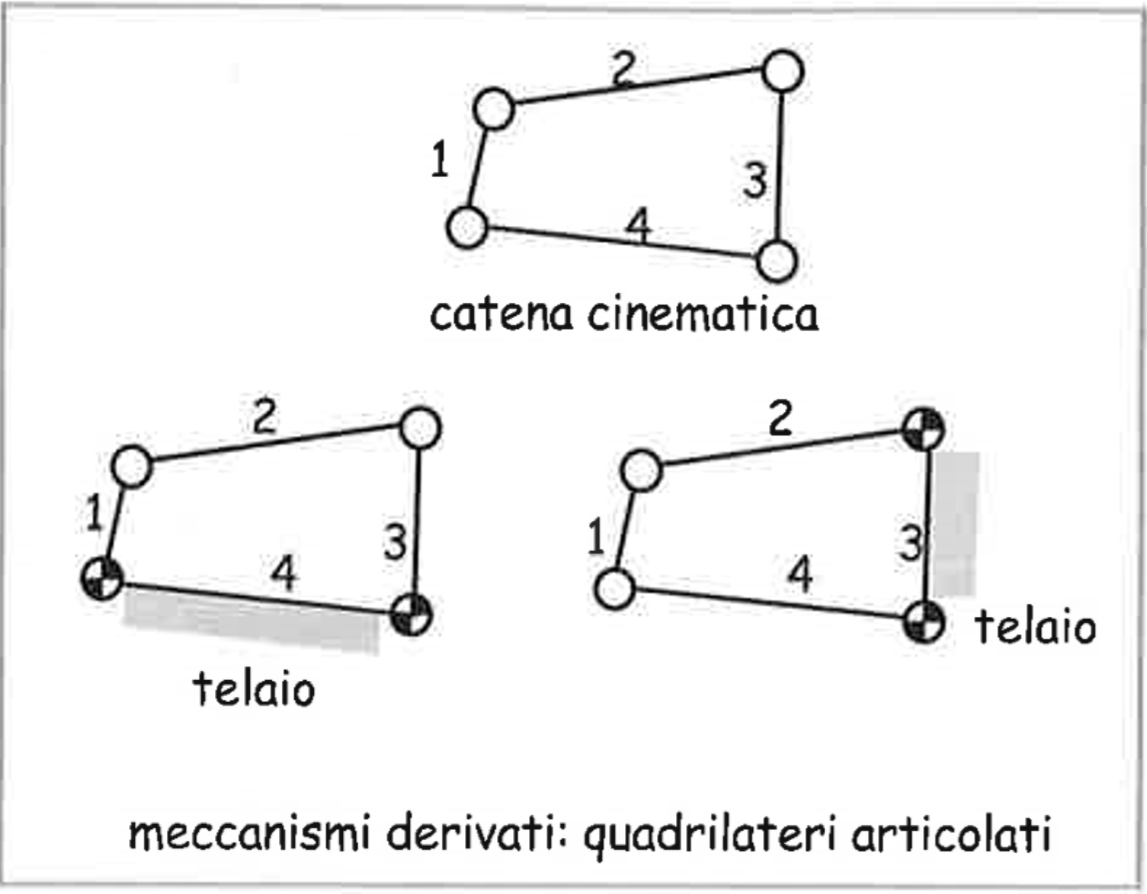
\includegraphics[width = 0.35\textwidth]{chapter02/immagine15}
\end{SCfigure}

Tuttavia è possibile sostituire alcune coppie rotoidali con coppie prismatiche, ottenendo la relativa catena cineamtica a quadrilatero RRRP. Inoltre, se il membro binario con coppia rotoidale e prismatica avesse lunghezza nulla le due coppie cinematiche si confonderebbero/risulterebbero sovrapposte.
Ciò a dimostrare che è possibile ricondursi a catene cinematiche equivalenti a seconda dei casi, purché si rispetti la funzione e il movimento relativo dei membri. (La natura di una coppia cinematica può essere cambiata)

\begin{figure}[h]
\centering
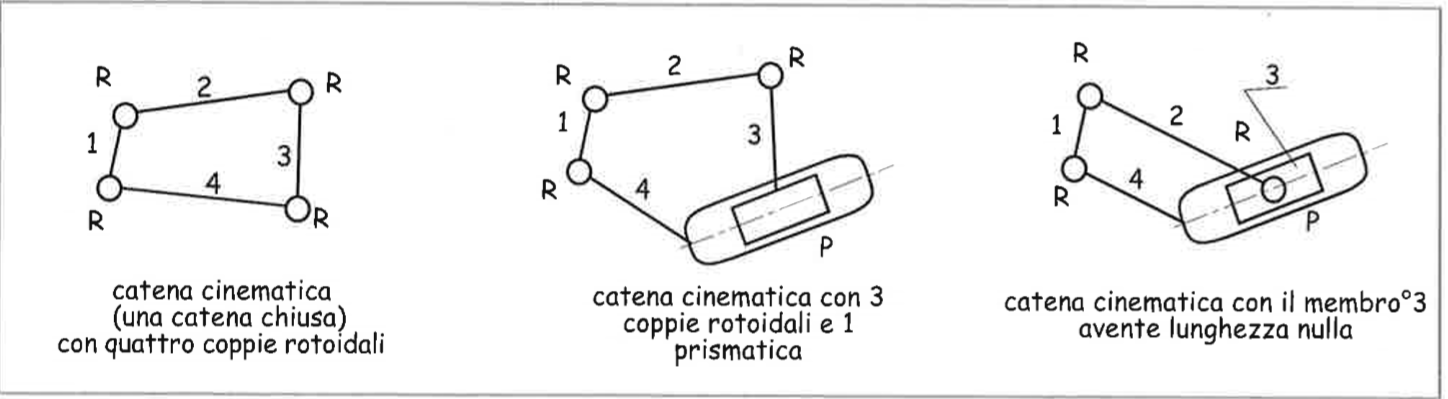
\includegraphics[width = 0.8\textwidth]{chapter02/immagine16}
\end{figure}

La catena cinematica appena ottenuta può, a questo punto, essere analizzata per scoprirne le funzioni che può compiere a seconda di quale membro venga posto a telaio.

\begin{figure}[h]
\centering
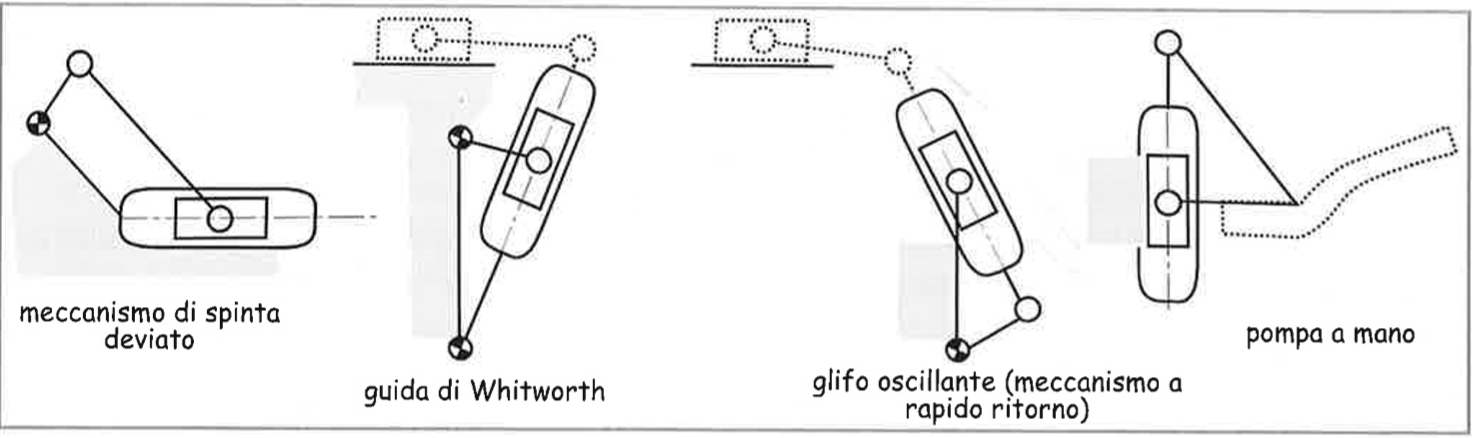
\includegraphics[width = 0.6\textwidth]{chapter02/immagine17}
\end{figure}

Il meccanismo di spinta deviato corrisponde ad un meccanismo a catena a quadrilatero chiuso in cui il perno della manovella non è sull'asse del pattino; l'utilità di tale meccanismo è da ricercarsi nella diversa lunghezza dell'arco di compressione e espasione.\newline
Più nel dettaglio il \textbf{meccanismo di spinta} deviato è costituito dal telaio collegato ad una manovella (capace di compiere un giro completo attorno ad una coppia rotoidale fissa) e da una biella collegata alla manovella tramite coppie rotoidali mobili. 
Il moto della  biella viene dunque trasferito ad un pattino o corsoio che, data la coppia prismatica (pattino) in cui è inserito, converte il moto rotazionale degli elementi precedenti in un moto lineare.


Per quanto riguarda le catene cinematiche a 6 corpi/membri, le più importanti sono da attribuire a Watt e Stephenson.
Di seguito vengono propoosti alcuni meccanismi derivanti dall'esalatero di Watt e Stephenson:

\begin{itemize}
\item {\scshape{\bfseries Esalatero di Watt e rispettivi meccanismi}}
\begin{figure}[h]
\centering
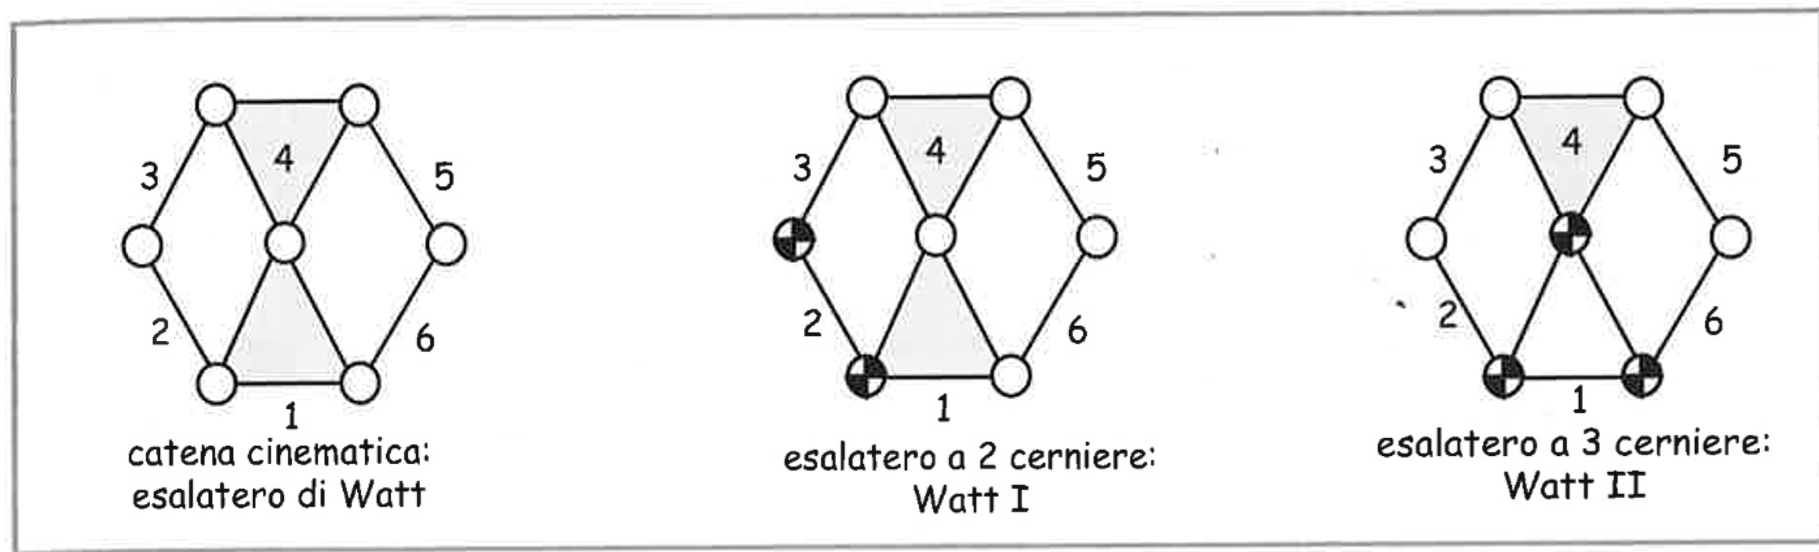
\includegraphics[width = 0.65\textwidth]{chapter02/immagine18}
\end{figure}\newline
I 6 corpi/membri che compongono l'esalatero di Watt sono collegati vicendevolmente da 2 coppie ternarie e 2 coppie binarie.\newline
In particolare i due corpi ternari sono collegati tra di loro e i due quadrilateri sono collegati in sequenza.
 
\item {\scshape{\bfseries Esalatero di Stephenson e rispettivi meccanismi}}

\begin{figure}[!h]
\centering
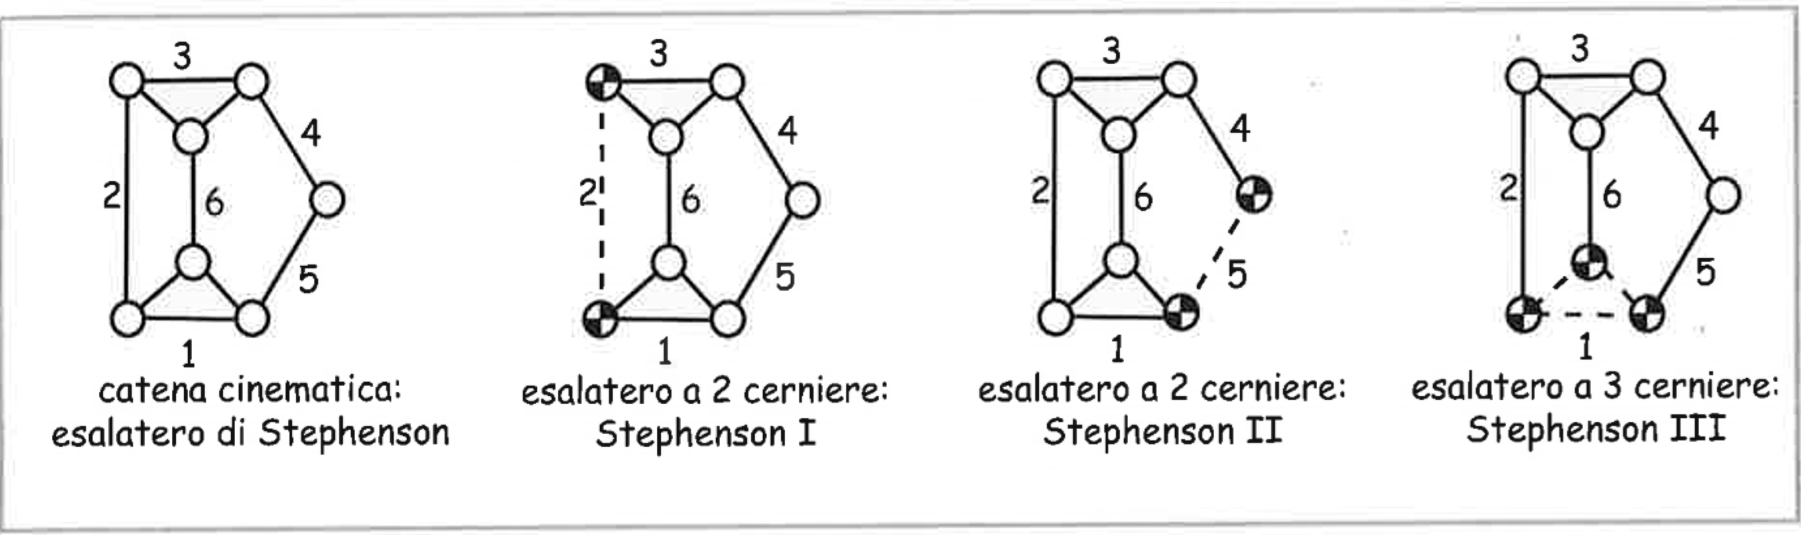
\includegraphics[width = 0.65\textwidth]{chapter02/immagine19}
\end{figure}

I 6 corpi/membri che compongono l'esalatero di Stephenson sono collegati vicendevolmente da 2 coppie ternarie e 2 coppie binarie. \newline
Tuttavia a differenza dell'esalatero di Watt i due corpi ternari non risultano essere collegati tra di loro direttamente, bensì vi è presente un corpo binario a svolgere tale funzione.
\end{itemize}

Fino ad ora sono stati affrontati dei meccanismi rappresentativi in maniera convenzionale mediante i loro schemi cinematici; nella realtà la realizzazione costruttiva potrebbe essere assai diversa dal corrispondente schema cinematico (\emph{e non immediatamente identificabile}).\newline
Un esempio di tale problema di identificazione può essere ricercato nel \textbf{giunto di Oldham}, che viene generalmente impiegato per trasmettere il moto tra due assi paralleli disallineati (aka \textbf{Giunto omocinetico}), e di cui è proposta una rappresentazione di seguito.

\begin{figure}[h]
\centering
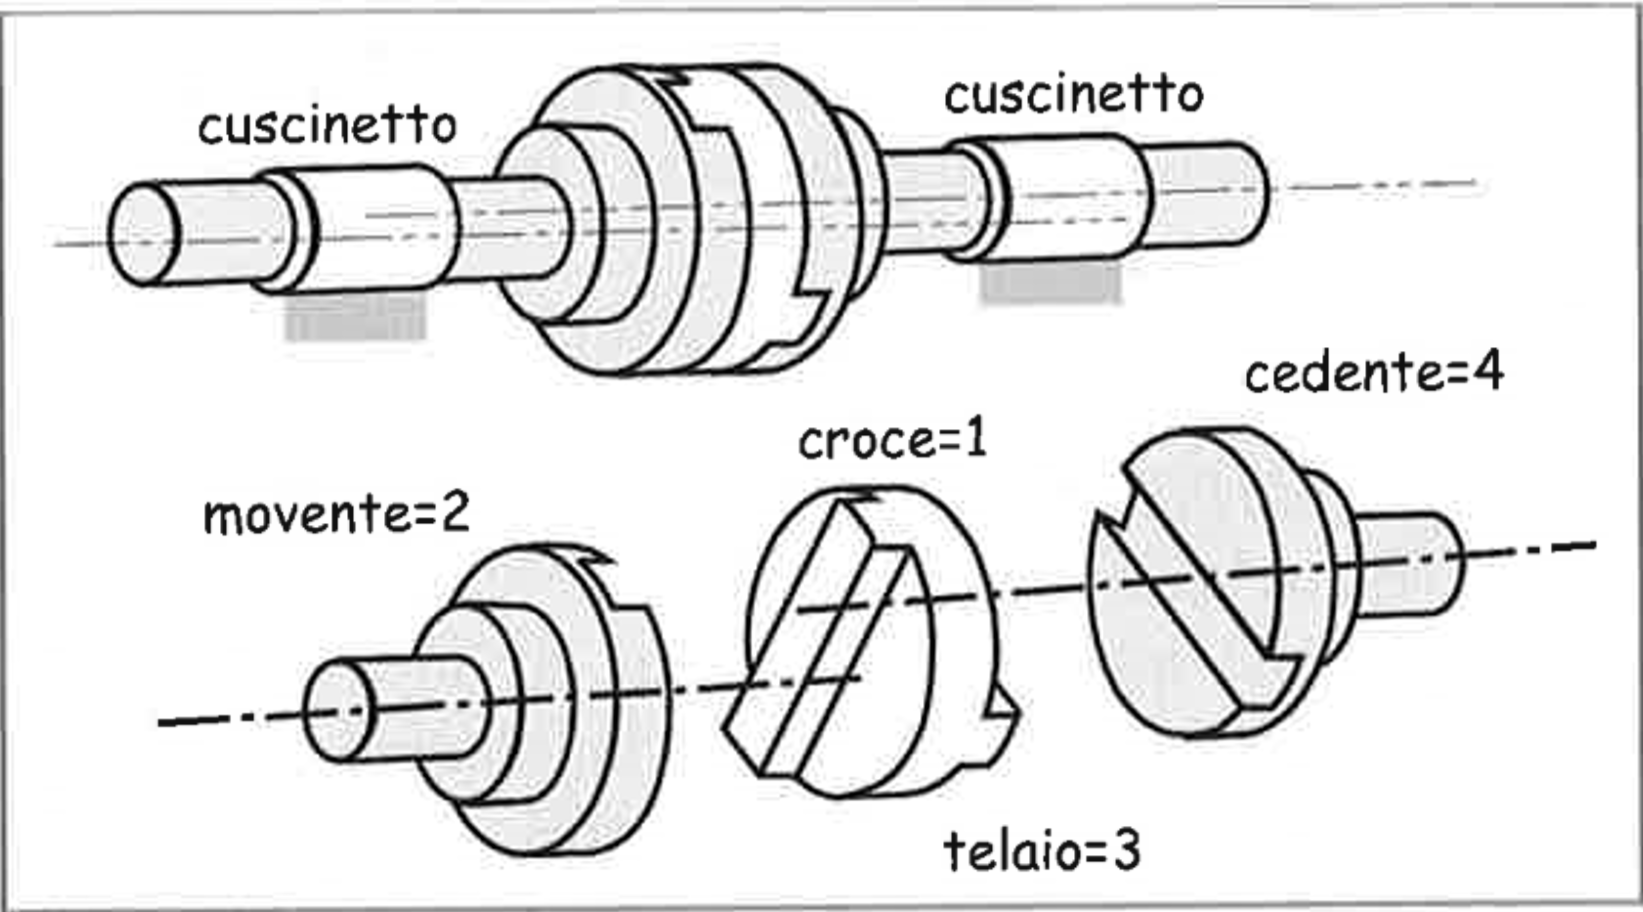
\includegraphics[width = 0.7\textwidth]{chapter02/immagine20}
\end{figure}

Infatti se volessimo rappresentare lo schema cinematico che descrive questo particolare giunto, esso si comporrebbe di un glifo a croce con l'asta 3 fissata al telaio, il pattino 2 e 4 (rispettivamente movente e cedente) e la croce 1 rappresentata dal corpo intermedio.

\begin{figure}[h]
\centering
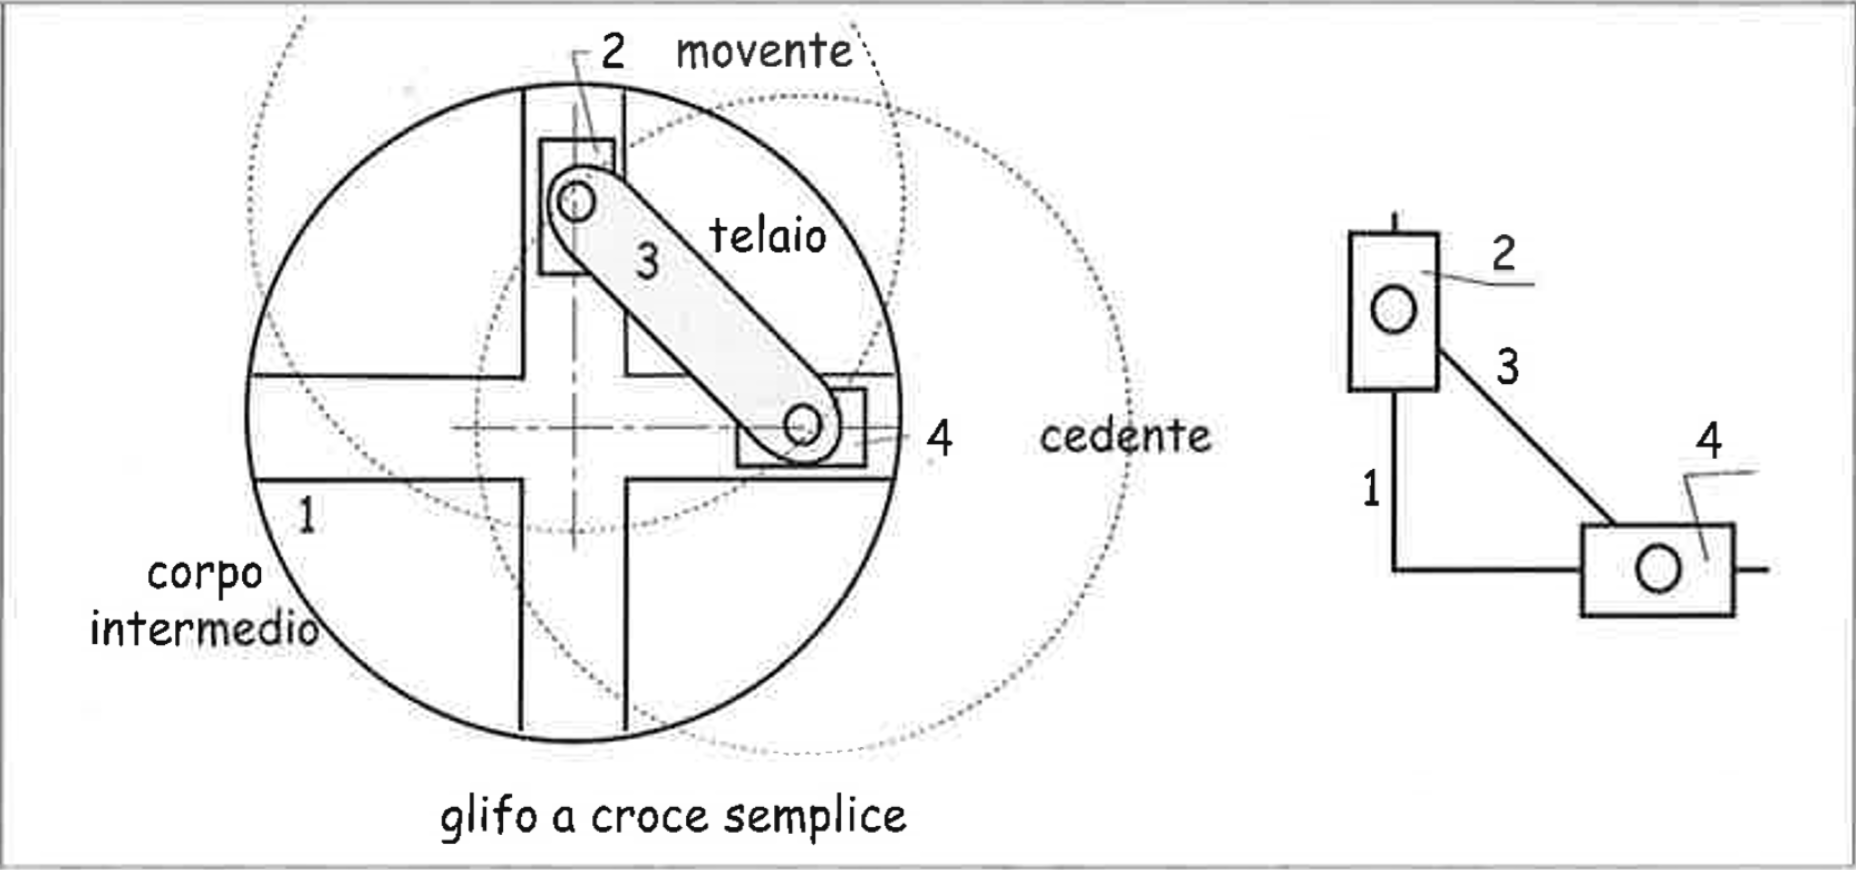
\includegraphics[width = 0.75\textwidth]{chapter02/immagine21}
\end{figure}


In futuro avremo molto a che fare con moventi e cedenti nella rappresentazione degli schemi cinematici. 
Di conseguenza risulta fondamentale darne subito una definizione:
\vspace{2mm}

{\scshape{\bfseries moventi del meccanismo}} (\emph{membri motori}) := membri sui quali agiscono delle forze esterne che compiono lavoro positivo detto lavoro motore (corpo di una catena cinematica a cui è imposto un movimento)

{\scshape{\bfseries cedenti del meccanismo}} (\emph{membri condotti}) := membri sui quali agiscono delle forze esterne che compiono lavoro negativo detto lavoro resistente (corpo di una catena cinematica che impone il movimento)
\vspace{2mm}

Ad esempio, nel meccanismo biella manovella azionato da un motore elettrico, il pistone/glifo rappresenta il cedente, il motore elettrico il movente.
Nel sistema ad ingranaggi il cedente è reppresentato dal carico sostenuto da una fune collegata all'ultima ruota ad ingranaggi, il movente è rappresentata dalla prima ruota ad ingranaggi che trasmette la rotazione al treno di ingranaggi successivi.


\section{Gradi di libertà dei meccanismi piani}
	
	Nel decorso di questa sezione ci occuperemo della determinazione dei gradi di libertà di sistemi meccanici, vincolati da coppie cinematiche, tramite degli esempi:

	\begin{enumerate}
		\item {\scshape{\bfseries Esempio n.1}}

		\vspace{1mm}
		\begin{minipage}{.55\textwidth}
			Il sistema in figura è composto da 3 corpi/membri:
			\begin{itemize}
			\item Il telaio 1 che non conferisce al sistema alcun G.d.L. (0 G.d.L.)
			\item Il corpo 2 che è collegato al telaio tramite una coppia rotoidale (R) e di conseguenza presenta un solo G.d.L. (1 G.d.L.)
			\item Il corpo 3 anch'esso collegato al corpo 2 tramite una coppia rotoidale (R) ed è, di conseguenza, denotato da un solo G.d.L. (1 G.d.L.)
			\end{itemize}
			\end{minipage}
			\hfill
			\begin{minipage}{.45\textwidth}
			\centering
			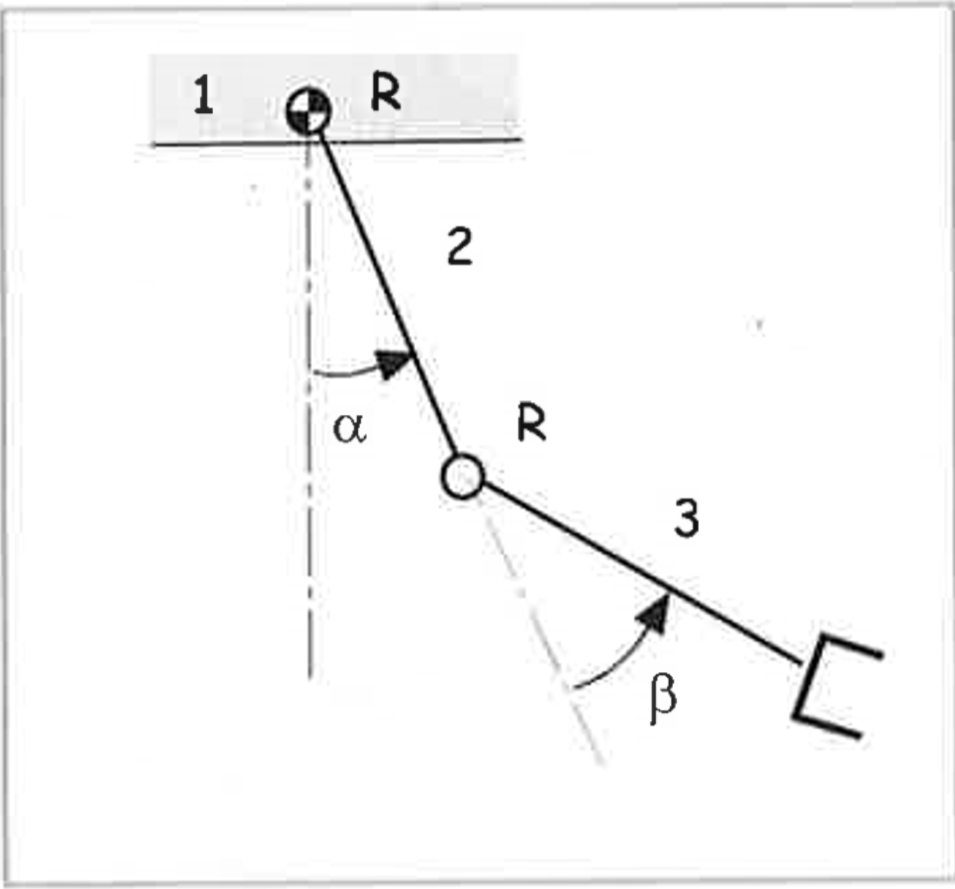
\includegraphics[width = .6\textwidth]{chapter02/immagine22}
			\end{minipage}
			
			In totale il meccanismo in questione presenta 2 G.d.L. che possono essere ricondotti agli angoli $\alpha$ (descrive la rotazione di 2 rispetto a 1) e $\beta$ (descrive la rotazione di 3 rispetto a 2).
			\newline
			Tali coordinate risultano essere 2 coordinate generalizzate, ovvero sufficienti e indipendenti a descrivere completamente il sistema di corpi.
		
			\item{\scshape{\bfseries Esempio n.2}}\newline
				Sostituendo all'esempio precedente la coppia rotoidale respondabile del collegamento tra i membri 2 e 3 con una coppia a camma (C) si libera un ulteriore G.d.L. del sistema, più in particolare di traslazione del corpo 3 rispetto a 2.\newline
				\begin{minipage}{.55\textwidth}
				In tal modo si potranno osservare 3 G.d.L. del meccanismo:
				\begin{itemize}
					\item Il telaio 1 che non conferisce al sistema alcun G.d.L. (0 G.d.L.)
					\item Il corpo 2 che è collegato al telaio tramite una coppia rotoidale (R) e di conseguenza denota un solo G.d.L. (1 G.d.L.)
					\item Il corpo 3 che è collegato al corpo 2 tramite una coppia a camma, di classe $c_2$, che conferisce al corpo 3 di ruotare attorno alla coppia stessa e di traslare (2 G.d.L.)
				\end{itemize}
				\end{minipage}
				\hfill
				\begin{minipage}{.45\textwidth}
					\centering
					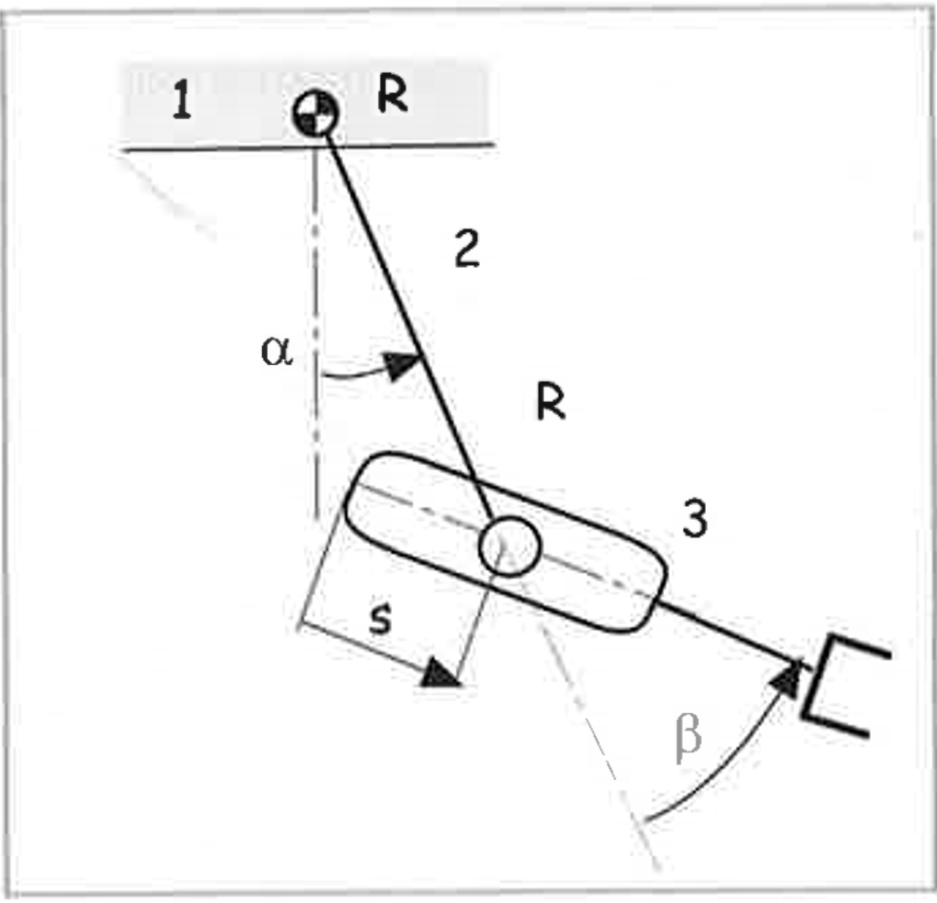
\includegraphics[width = .6\textwidth]{chapter02/immagine23}
				\end{minipage}

				Le coordinate generalizzate del sistema in esame saranno, di conseguenza:
				$\alpha$, $\beta$ (cfr. Esempio n.1) e \emph{s} (= traslazione rispetto ad un estremo della coppia prismatica in cui è presente la camma) (tutte funzioni del tempo: $\alpha$(t), $\beta$(t) e \emph{s}(t))
				e  risultano, difatti, parametri sufficienti e  necessari a descrivere completamente la posizione del sistema meccanico
		\item {\scshape{\bfseries Esempio n.3}}\newline
		La catena cinematica chiusa, anche conosciuta con il nome di meccanismo di spinta deviato, e riportata a fianco, si compone di 4 membri/corpi, che se considerati indipendenti contribuiscono al calcolo con 3 G.d.L. ciascuno ($4 (membri) \cdot 3 (G.d.L.) = \textbf{12} (\textbf{G.d.L})$):
	
		\begin{itemize}
			\item Il corpo 1 (manovella) che è collegato al telaio e al corpo 2 tramite 2 coppie rotoidali (R) e priva il sistema di 2 G.d.L
			\item Il corpo 2 (biella) che è collegato ai corpi 1 e 3 tramite coppie rotoidali (R) (- 2 $\cdot$ 3 = \textbf{- 6 G.d.L.})
			\item Il corpo 3 (pistone) che trasforma il moto rotoidale dei corpi precedenti in un moto lineare ed è collegata al telaio tramite una coppia prismatica che priva il sistema di 2 G.d.L. (\textbf{- 2 G.d.L} $\cdot$ 1)
			\item Il corpo 4 (telaio) che rappresenta la sede entro cui avviene la traslazione del pistone e priva il sistema di 3 G.d.L. (\textbf{- 3 G.d.L.})
		\end{itemize} 
		
			\begin{figure}[h]
		\centering
		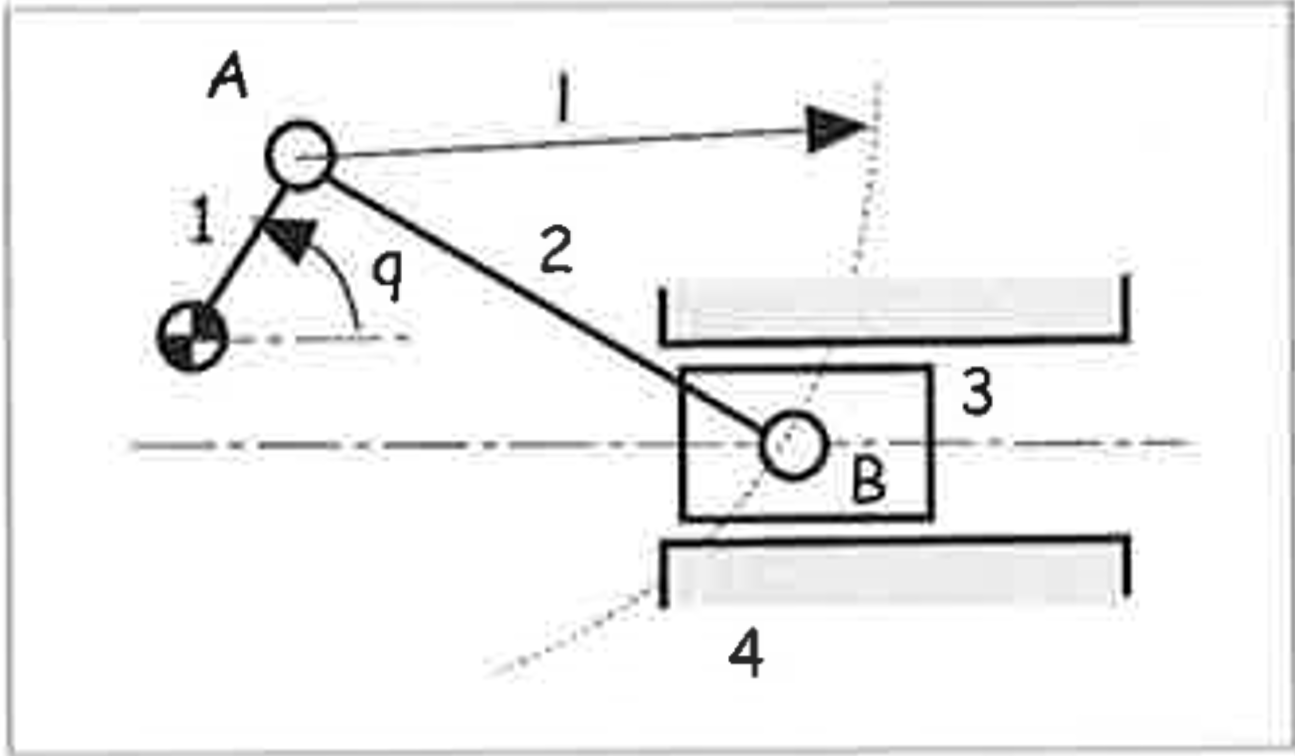
\includegraphics[width = .25\textwidth]{chapter02/immagine24}
		\end{figure}
		
		In conclusione possiamo determinare il numero di G.d.L. del meccanismo nel seguente modo:
		\begin{equation*}
		12\emph{(corpi indipedenti)} - 3 (telaio) - 6 (R) - 2 (P) = 1 (G.d.L.) 
		 \end{equation*}
		
		\begin{minipage}{.6\textwidth}
		Infatti si può osservare che la posizione e il movimento del meccanismo può essere descitto da un' unica coordinata generalizzata, ad esempio l'angolo rispetto all'orizzontale \emph{q(t)} che la manovella individua attorno il telaio, oppure la posizione del pistone/glifo ripetto alla sua condizione iniziale \emph{x(t)}.
		\end{minipage}
		\hfill
		\begin{minipage}{.4\textwidth}
		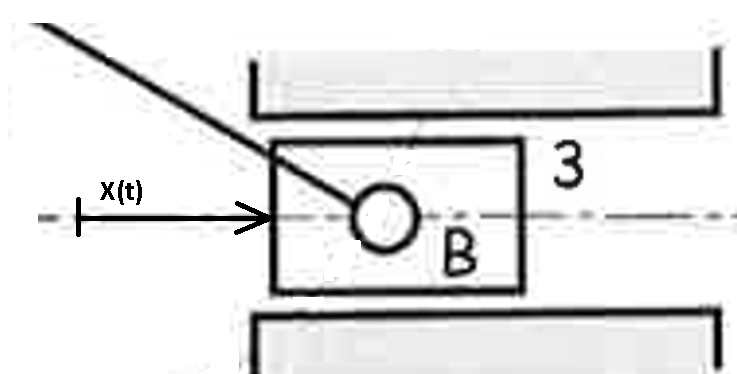
\includegraphics[width = .7\textwidth]{chapter02/immagine25}
		\end{minipage}
		
		\begin{minipage}{.25\textwidth}
			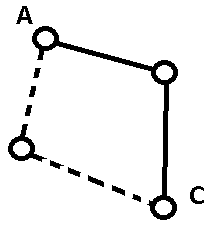
\includegraphics[width=1\textwidth]{chapter02/immagine26}
		\end{minipage}
		\hfill
		\begin{minipage}{.65\textwidth}
		Ciò che non viene tenuto in considerazione è che in questo particolare esempio esistono in realtà due soluzioni ammesse/configurazioni:\newline
		Infatti in catene cinematiche chiuse esistono più modi per calcolare il meccanismo.\newline
		 Una volta date le posizioni del punto/coppie di punti A e C, esistono due modi di chiudere la catena cineamtica.
		\end{minipage}
		\vspace{3mm}
		
		Il metodo appena utilizzato per la determinazione dei G.d.L. del meccanismo prende il nome di  \textbf{Equazione di Gr\"ubler} e risulta applicabile a meccanismi piani in catena chiusa.
		Il processo iterativo che sta alla base di questo metodo si basa sui seguenti step:
		\begin{itemize}
		\item Ogni corpo/membro indipendente dal sistema, contribuisce al calcolo dei G.d.L. del meccanismo introducendo 3 G.d.L. ciascuno (se il corpo appartiene al piano)
		\item Sottrarre i 3 G.d.L. che il telaio, essendo fisso, priva.
		\item Sottrarre i 2 G.d.L per ogni coppia di classe $c_1$ che vincola il sistema di corpi lasciando libero 1 G.d.L., ovvero coppie prismatiche (P) e coppie rotoidali (R)
		\item Sottrarre 1 G.d.L. per ogni coppia di classe $c_2$ che vincola il corpo lasciando liberi 2 G.d.L., ovvero la coppia a camma (C)  
 		\end{itemize} 
 		
 		E può essere sintetizzato enunciando la seguente formulazione:
 		\begin{equation}
 		n = 3m - 2c_1 - c_2
 		\end{equation}
		se il sistema in questione è una catena cinematica piana (1)
		\begin{equation}
		n = 3(m-1) -2c_1 - c_2
		\end{equation}
		nel caso di meccanismi piani (2).%
		\footnote{La prinipale differenza tra le due equazioni risiede nella presenza o meno di un telaio che sottrae al calcolo 3 G.d.L. }
	
		
		
		I parametri che compongono tali formule sono:
		\begin{equation*}
			\begin{split}
				\textbf{n} &= \emph{numero di G.d.L. del sistema di corpi}\\
				\textbf{m} &= \emph{numero di membri/corpi che compongono il sistema}\\
				&\emph{(dove il ``-1''  considera i G.d.L. che il telaio rimuove)}\\
				\textbf{$2 \cdot c_1$} &= \emph{indica il numero di G.d.L. (2) che il numero di coppie di classe $c_1$ privano}\\
				\textbf{$c_2$} &= \emph{indica il numero di G.d.L (1) che il numero di coppie di classe $c_2$ privano}
			\end{split}
		\end{equation*}
		
	\end{enumerate}
	
	Affrotiamo più nel dettaglio l'utilità e i limiti dell'equazione di Gr\"ubler con i seguenti esempi:
	\begin{itemize}
	\item \textbf{Catene cinematiche chiuse con 3 corpi}\newline
	\begin{minipage}{.25\textwidth}
	\centering
	 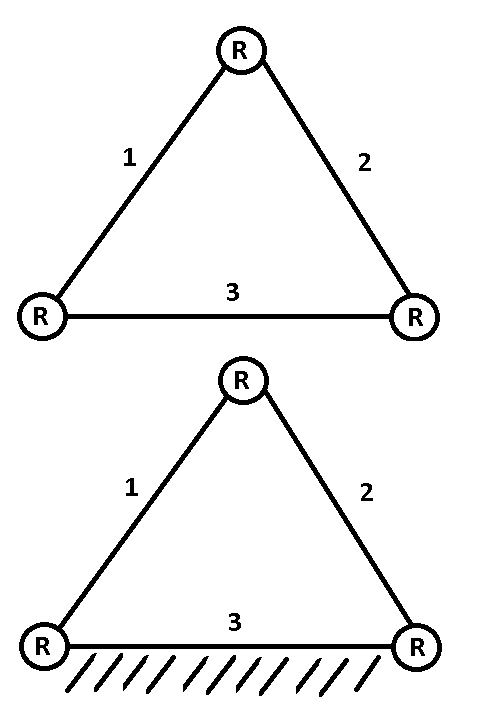
\includegraphics[width = .65\textwidth]{chapter02/immagine27}
	 \end{minipage}
	 \hfill
	 \begin{minipage}{.75\textwidth}
		\[n = 3 \cdot (3) - 2 \cdot 3 = 9-6 = 3 \emph{G.d.L.}\]
		\emph{ (la catena cinematica è libera di muoversi nel piano)}
		\vspace{3mm}
		
		\[n = 3 \cdot (3 - 1) -2 \cdot 3 = 0 \emph{ G.d.L. }\]
		\emph{(una volta definito un telaio tale accoppiamento dei tre corpi assume il valore di una struttura)}

	\end{minipage}
		
		\item \textbf{Catene cinematiche a 5 corpi}
		\vspace{1mm}
		
			\begin{minipage}{.25\textwidth}
			\centering
				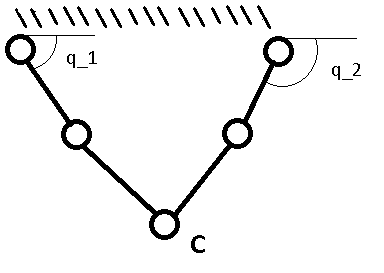
\includegraphics[width = .75\textwidth]{chapter02/immagine28}
			\end{minipage}
			\hfill
			\begin{minipage}{.65\textwidth}
			\begin{equation*}
			n = 3 \cdot (5 - 1) - 2 \cdot 5 = 12- 10 = 2 \emph{G.d.L.}
			\end{equation*}

			Il pentalatero in questione, su cui si basano i manipolatori paralleli, una vota che vengono determinati $q_1$ e $q_2$, permette il controllo della posizione del punto C
						\end{minipage}		
			\item  \textbf{Catene cinematiche a 6 corpi}\newline
				Esalatero di Watt\newline
				\begin{minipage}{.25\textwidth}
					\centering
					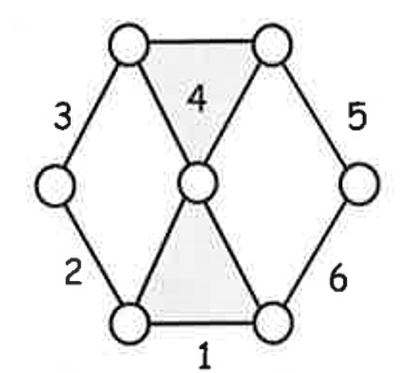
\includegraphics[width = .6\textwidth]{chapter02/immagine29}
				\end{minipage}
				\hfill
				\begin{minipage}{.75\textwidth}
				\begin{equation*}
					n = 3 \cdot (6 - 1) - 2 \cdot 7 = 15-14 = 1 \emph{G.d.L.}
				\end{equation*}
				\end{minipage}
				
				Giunto di Oldham\newline
				\begin{minipage}{.25\textwidth}
					\centering
					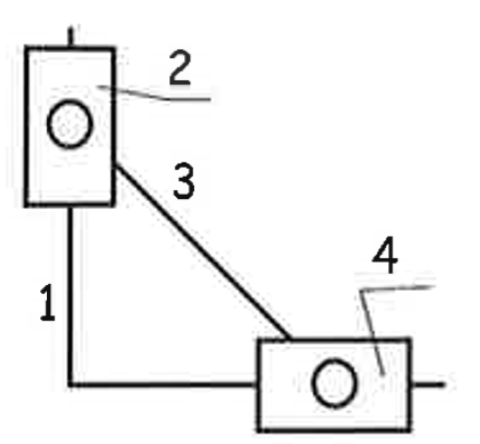
\includegraphics[width = .6\textwidth]{chapter02/immagine30}
				\end{minipage}
				\hfill
				\begin{minipage}{.75\textwidth}
				\begin{equation*}
					n = 3 \cdot (4 - 1) - 2 \cdot 4 = 9 - 8 = 1 \emph{G.d.L.}
				\end{equation*}
				\end{minipage}
		
	\end{itemize}
	\newpage
	
	Tuttavia la formula di Gr\"ubler non considera alcuni casi:
	\begin{enumerate}
	\item {\scshape{\bfseries Caso 1}} \newline
		Consideriamo il seguente sistema a 6 corpi (esalatero) i cui accoppiamenti sono eseguiti da 6 coppie (4 rotoidali e 2 prismatiche) di classe $c_1$.
		Utilizzando la formula di Gr\"ubler per determinare il numero di G.d.L. di tale meccanismo si ottiene un risultato scorretto:
\begin{figure}[h]
\centering
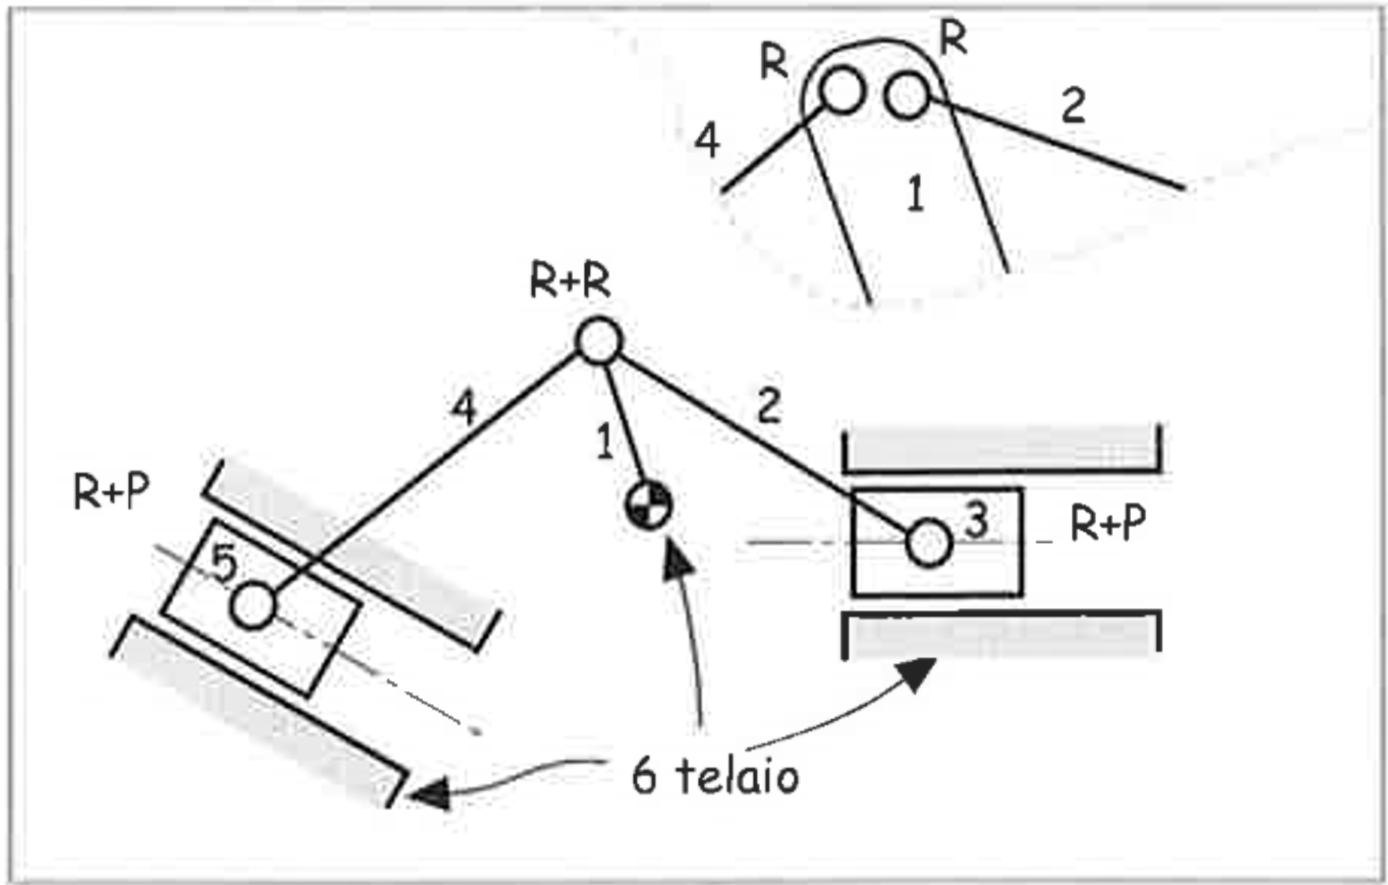
\includegraphics[width = .5\textwidth]{chapter02/immagine31}
\end{figure}
		\begin{equation*}
			n = 3 \cdot (6 - 1) - 2 \cdot 6 = 15 - 12 = 3  \emph{G.d.L.} 
		\end{equation*}
	Tuttavia, si può notare che scegliendo una variabile \emph{q} come coordintata generalizzata, la posizione del punto B viene completamente identificata e, di conseguenza, anche la posizione degli altri membri è identificata.
	 
	 La ragione per cui la formula di Gr\"ubler abbia ritornato un risultato sbagliato pur da una corretta identificazione dei membi appartenenti al sistema e delle coppie a loro applicate è da ricercarsi al punto B: infatti la coppia rotoidale che è applicata nel punto B e che lega i corpi 1, 2 e 4 deve essere contata 2 volte.
	 \begin{equation*}
	 	n = 3 \cdot (6 - 1) - 2 \cdot 7 = 1 \emph{G.d.L.}
	 \end{equation*}
	
	Non a caso il meccanismo proposto è equivalente ad un esalatero di Watt
	
	\item {\scshape{\bfseries Caso 2}} \newline
		Consideriamo il seguente sistema formato da due manovelle e una biella, e immaginiamo di introdurre a metà della biella una coppia rotoidale che lega un ulteriore corpo a telaio.
		\begin{figure}[h]
		\centering
		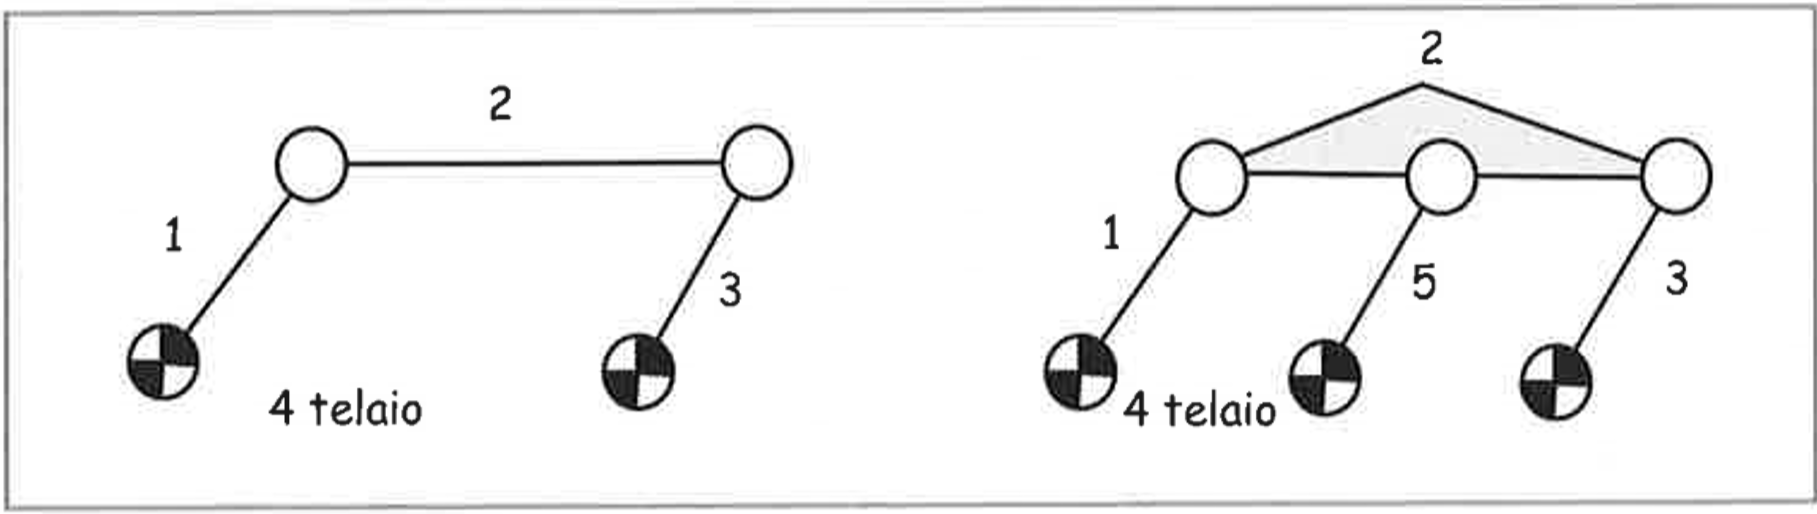
\includegraphics[width = .5\textwidth]{chapter02/immagine32}
		\end{figure}
		
		Dal calcolo dei G.d.L. ramite la formula di Gr\"ubler si ottiene un risultato errato:
		\begin{equation*}
			n = 3 \cdot (5 - 1) - 2 \cdot 6 = 12 - 12 = 0 \emph{G.d.L}
		\end{equation*}
		
		Questo meccanismo dovrebbe avere 0 G.d.L. seguendo la relazione di Gr\"ubler, tuttavia tutti i punti della biella centrale descrivono una circonferenza attorno alla coppia R del telaio adiacente (membro 4).
		Ho aggiunto cioè dei vincoli non necessari che il meccanismo originale già aveva in quanto poteva compiere già una rotazione (manovelle 1 e 3) attorno al telaio
		
		In sintesi: la manovella 5, che è parallela alla 1 e alla 3, non aggiunge alcun vincolo addizionale al movimento del membro 2.
		La formula di Gr\"ubler pur essendo stata applicata in maniera corretta non considera che le coppie aggiunte possono non introdurre vincoli al moto del meccanismo.

	\item {\scshape{\bfseries Caso 3}} \newline
	Considerando il glifo a croce composto il numero di gradi di libertà che si ottengono dall'applicazione della formula di Gr\"ubler è:
	\begin{equation*}
		n = 3 \cdot (5 - 1) - 2 \cdot 6 = 12 - 12 = 0 \emph{G.d.L.} 
	\end{equation*}
	\begin{figure}[h]
	\centering
	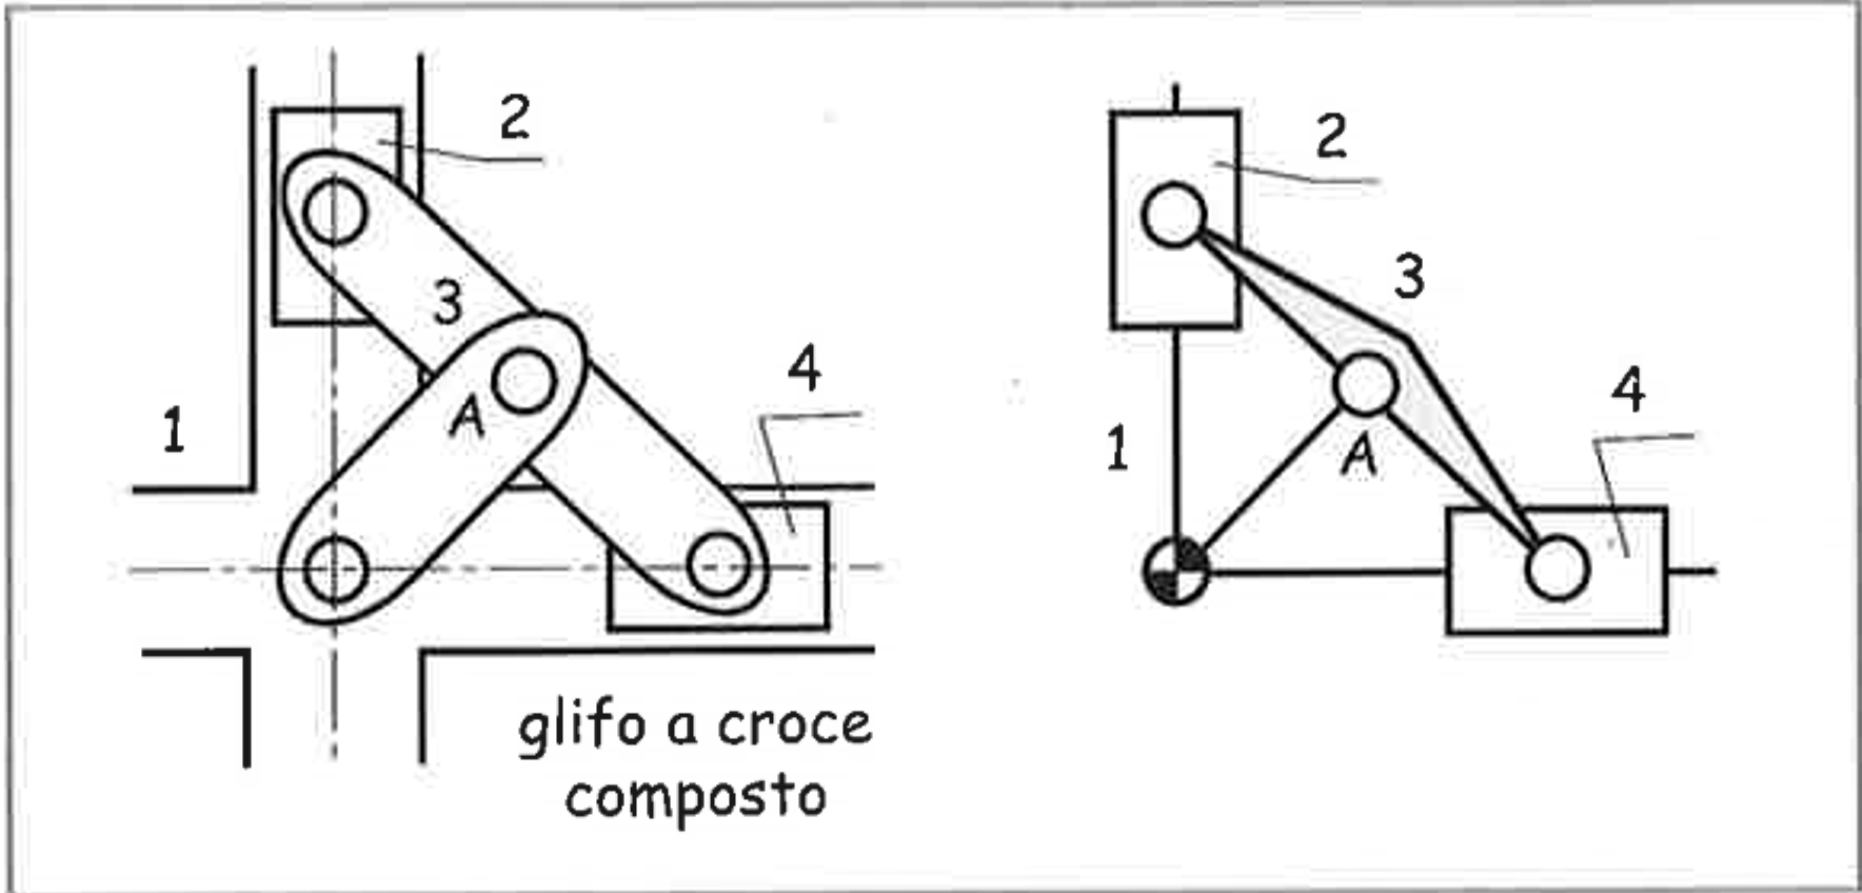
\includegraphics[width = .5\textwidth]{chapter02/immagine33}
	\end{figure}
	
	Tuttavia, analogamente al caso precedente, l'aggiunta del corpo in A non introduce vincoli aggiuntivi al movimento del meccanismo, in quanto A, sia prima che dopo l'introduzione del corpo, descriveva una traiettoria circolare avente come centro il punto di intersezione dei due assi di scorrimento.
		\end{enumerate}
	
	Osservazioni conclusive:
	\begin{itemize}
	\item Spesso nei meccanismo abbiamo anche degli elementi elastici quali molle; questi elementi elastici non modificano la possibilità di movimento ma fanno nascere delle forze.\newline
	Ad esempio una molla non modifica i G.d.L. del meccanismo di spinta perché essa può allungarsi o accorciarsi. Possiamo quindi ignorarle quando scriviamo l'equazione di Gr\"ubler.
	\item In altri casi dei membri rigidi sono connessi da elementi deformabili che permettono la trasmissione del moto (\emph{ad esempio cinghie e funi}). In tal caso il numero di G.d.L. può essere facilmente determinato facendo delle ipotesi semplificate.\newline
	Se si ipotizza che la cinghia sia inestensibile e non presenti scorrimenti la ruota 3 si muove insieme alla ruota 1 e quindi il sistema ha un solo G.d.L.
	\begin{figure}[h]
	\centering
	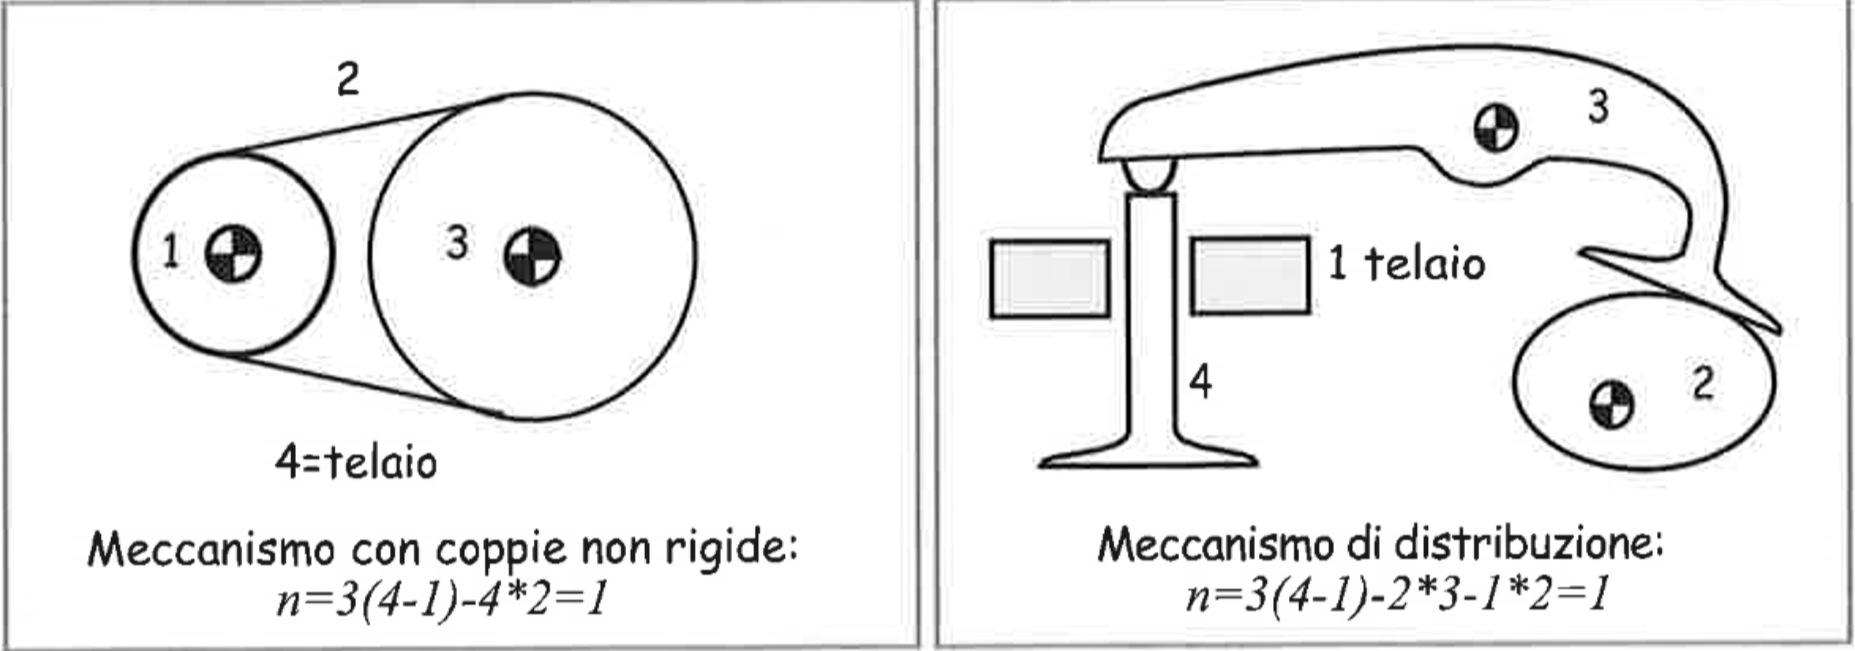
\includegraphics[width = .5\textwidth]{chapter02/immagine34}
	\end{figure}
	\item Di seguito sono riportati alcuni esempi di applicazione della equazione di  Gr\"ubler.\newline
	\begin{figure}[h]
	\centering
	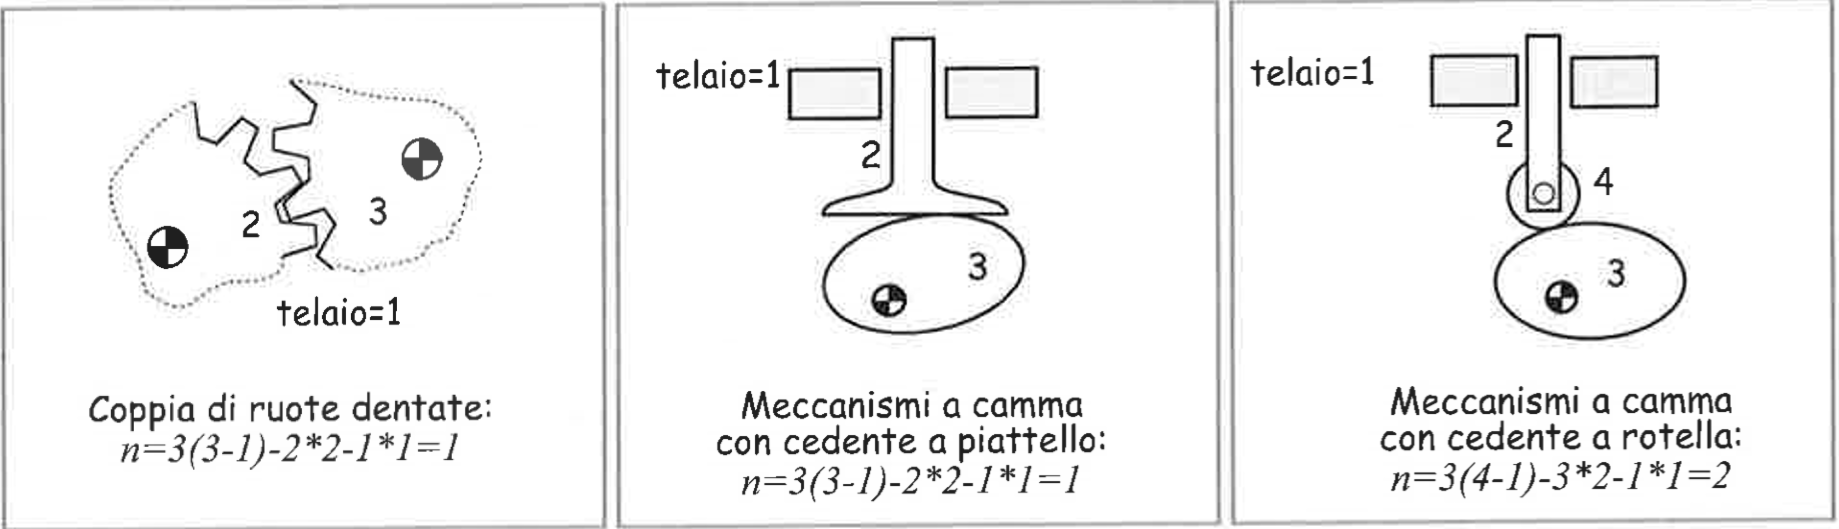
\includegraphics[width = .65\textwidth]{chapter02/immagine35}
	\end{figure}
		\end{itemize}

	\section{Cinematica dei corpi rigidi}
		\subsection{Introduzione}
		
			Al variare del tipo di problema da studiare gli organi costituenti le macchine possono venire schematizzati come dei punti materiali, dei corpi rigidi, dei sistemi di corpi rigidi, dei corpo deformabili. Una delle schematizzazioni più importanti è quella di corpo rigido; ne richimiamo quindi le relazioni fondamentali della cinematica.
		
			Procediamo, dunque, a definire alcuni elementi che saranno di utilità nel decorso della trattazione di tali relazioni:
		
			\begin{minipage}{.55\textwidth}
				\centering
				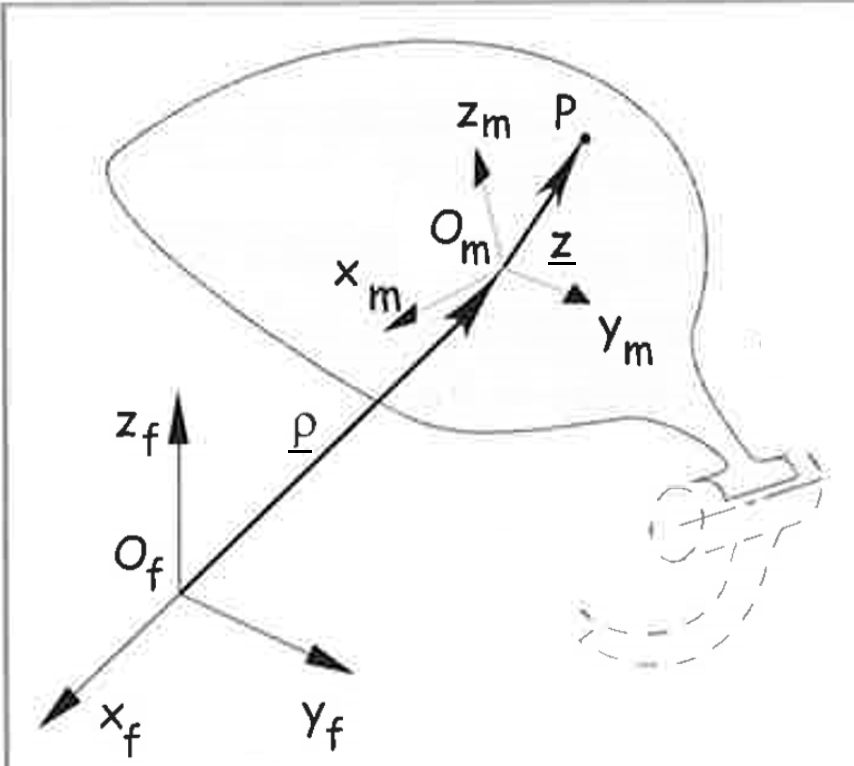
\includegraphics[width = .75\textwidth]{chapter02/immagine36}
			\end{minipage}
			\hfill
			\begin{minipage}{.45\textwidth}
				\begin{itemize}
					\item  \textbf{Terna mobile}:  una terna solidale al corpo stesso individuata dai versori ($\mathbf{i_m}, \mathbf{j_m}, \mathbf{k_m}$), e dalle generiche coordinate ($x_m, y_m, z_m$) in cui viene esplicitato il pedice ``m'' in riferimento al fatto che sono solidali alla terna mobile.
					\item \textbf{Terna fissa}: una terna di versori ($\mathbf{i_f}, \mathbf{j_f}, \mathbf{k_f}$) e coordinate generiche  ($x_f, y_f, z_f$)  in cui viene esplicitato il pedice ``f'' in riferimento al fatto che sono solidali ad un osservatore inerziale.
					\item \textbf{Un punto P} solidale alla terna mobile.
					\item il vettore $\und{\rho}$ che identifica la distanza della terna mobile dalla terna fissa
					\item il vettore $\mathbf{z}$ che identifica la distanza del punto P dalla terna mobile
				\end{itemize}
			\end{minipage}
			\vspace{1mm}
		
				Si è interessati a trovare le coordinate del punto P in un sistema di riferimento assoluto, ovvero le coordinate del punto P rispetto alla terna fissa ($\mathbf{O_fP}$): bisognerà risolvere l'equazione vettoriale:
			\begin{equation*}
				\begin{split}
					\mathbf{O_fP} &= \mathbf{O_fO_m} + \mathbf{O_mP}\\
					\mathbf{P} &= \underline{\rho} + \mathbf{z}
				\end{split}
			\end{equation*}

			Osservazioni: 
			\begin{enumerate}[$\rightarrow$]
				\item $\mathbf{O_mP}$ sono le coordinate del punto P rispetto all'origine della terna mobile e possono essere esplicitate come combinazione lineare dei versori della stessa terna, ovvero:
					\begin{equation*}
						\mathbf{O_mP} = \quad ^mx_P \cdot \mathbf{i_m} +\quad ^my_P \cdot \mathbf{j_m} +\quad ^mz_P \cdot \mathbf{k_m}
					\end{equation*}
				\item Introducendo la nozione di corpo rigido le coordinate relative di qualsiasi punto rispetto ad un sistema di riferimento solidale all'oggetto sono fisse / costanti. Di conseguenza, le coordinate ($ ^m\!x_P, ^m\!y_P, ^m\!z_P$) sono per l'ipotesi di corpo rigido, costanti durante tutto il moto.
				\item \textbf{Corpo rigido} (Definizione \#1): sistema di punti materiali che hanno coordinate costanti in un sistema di riferimento solidale con il corpo stesso.
				\item \textbf{Corpo rigido} (Definizione \#2): insieme di punti che a due a due hanno distanza costante.
				\item Per le ipotesi di corpo rigido che abbiamo appena posto al sistema, si può fare riferimento al moto del punto P come\textbf{ moto dello spazio rigido solidale alla terna mobile}
			\end{enumerate}
		
		\subsection{Velocità angolare}
			Siamo giunti a formulare la relazione vettoriale che lega la posizione di un punto rispetto ad una terna mobile alla sua posizione rispetto alla terna fissa, e abbiamo constatato che le coordinate del punto P solidale alla terna mobile sono costanti durante tutto il moto.
			
				\begin{equation*}
					\mathbf{O_fP} =  \underline{\rho} +  \, ^mx_P \cdot \mathbf{i_m} +\, ^my_P \cdot \mathbf{j_m} +\, ^mz_P \cdot \mathbf{k_m}
				\end{equation*}
		
		Procediamo ora a valutare una relazione che leghi la velocità del corpo (e quindi del punto P) rispetto all'osservatore assoluto/inerziale, eseguendo la derivata rispetto al tempo della relazione appena ottenuta:
		
				\begin{equation*}
					\dot{\mathbf{O_fP}} = \,^f\mathbf{v_P} = \dot{\underline{\rho}} + \,^mx_P \cdot \dot{\mathbf{i_m}} + \,^my_P \cdot \dot{\mathbf{j_m}} + \,^mz_P \cdot \dot{\mathbf{k_m}}
				\end{equation*}
		
		Per dare un significato fisico al risultato sopra esposto, rimane da determinare le derivate nel tempo dei tre versori della terna mobile:
		\[ \dot{\mathbf{i_m}} = \frac{d}{dt} \,{\mathbf{i_m}} \qquad ; \qquad \dot{\mathbf{j_m}} = \frac{d}{dt} \,{\mathbf{j_m}}  \qquad ; \qquad \dot{\mathbf{k_m}} = \frac{d}{dt} \,{\mathbf{k_m}} \]

		Considerando, ad esempio, il versore $\mathbf{k_m}$ (vettore di modulo unitario), il prodotto scalare per se stesso ritorna la norma al quadrato:
		\begin{equation*}
		\begin{split}
			\mathbf{k_m} \cdot \mathbf{k_m} &= \norma{k_m}^2 = 1\\
			\frac{d}{dt} (\mathbf{k_m} \cdot \mathbf{k_m}) &= \frac{d}{dt}(1)\\
			(\frac{d}{dt}\mathbf{k_m}) \cdot  \mathbf{k_m} +  \mathbf{k_m} \cdot (\frac{d}{dt}\mathbf{k_m}) &= 0\\
			2 (\frac{d}{dt}\mathbf{k_m}) \cdot \mathbf{k_m} &= 0
		\end{split}
		\end{equation*}
		
		La conclusione che possiamo trarre dallo sviluppo del versore in questione, e che può essere estesa anche ai rimanenti, è che: poiché il prodotto scalare $ \dot{\mathbf{k_m}} \cdot \mathbf{k_m}$ è nullo, i due vettori sono ortogonali.
		
		Fu Poisson a ipotizzare che esistesse un vettore tale per cui il suo prodotto vettoriale con il versore desse come risultato la derivata del versore. Come è noto, infatti, il prodotto vettoriale di due vettori non paralleli dà come risultato un vettore con direzione perpendicolare al piano che tali vettori individuano e verso definito dalla regola della mano destra.
		
		Rimane, dunque, da trovare i vettori ($\underline{\omega}^{(1)}, \underline{\omega}^{(2)}, \underline{\omega}^{(3)}$) tali per cui valgano le relazioni (anche conosciute come formule di Poisson):
		
		\[ \dot{\mathbf{i_m}} = \underline{\omega}^{(1)} \wedge{\mathbf{i_m}} \qquad ; \qquad \dot{\mathbf{j_m}} =\underline{\omega}^{(2)} \wedge {\mathbf{j_m}}  \qquad ; \qquad \dot{\mathbf{k_m}} = \underline{\omega}^{(3)} \wedge {\mathbf{k_m}} \]
		
		Per nostra fortuna Poisson si accorse che i vettori ($\underline{\omega}^{(1)}, \underline{\omega}^{(2)}, \underline{\omega}^{(3)}$) rappresentavano il medesimo vettore che, di conseguenza, prende il nome di vettore velocità angolare e a cui si farà riferimento, d'ora in poi, con il simbolo $\underline{\omega}$ in quanto il moto dei versori della terna mobile non è scorrelato.
		
		Perciò, per qualsiasi vettore unitario \textbf{solidale} al sistema di riferimento della terna mobile varrà l'uguaglianza vettoriale $ \frac{d}{dt} \,{\mathbf{u}} = \underline{\omega} \wedge \mathbf{u}$.
		
		Per quanto riguarda il moto di un vettore non necessariamente solidale alla terna mobile, si può eseguire un ragionamento analogo a quello fatto precedentemente:
		
		La posizione del vettore $\mathbf{u}$ può essere espressa come combinazione lineare delle sue coordinate rispetto ai versori della terna mobile:
			\[\mathbf{u} =  \, ^mu_x \cdot \mathbf{i_m} +\, ^mu_y \cdot \mathbf{j_m} +\, ^mu_z \cdot \mathbf{k_m}\]

		Mentre il suo moto è descritto dalla derivata totale rispetto al tempo dell'espressione appena ottenuta:
		
		\begin{equation*}
		\begin{split}
			\frac{d}{dt}\mathbf{u} &= \frac{d}{dt}(^mu_x) \cdot \mathbf{i_m} \quad + \quad \frac{d}{dt}(^mu_y) \cdot \mathbf{j_m} \quad + \quad \frac{d}{dt}(^mu_z) \cdot \mathbf{k_m}\\
							& + ^mu_x \cdot \frac{d}{dt}(\mathbf{i_m}) \quad + \quad ^mu_y \cdot \frac{d}{dt}(\mathbf{j_m}) \quad +\quad  ^mu_z \cdot \frac{d}{dt}(\mathbf{k_m})\\
\\
						&=  \dot{u_x} \cdot \mathbf{i_m} + \dot{u_y}\cdot \mathbf{j_m} + \dot{u_z} \cdot \mathbf{k_m} \quad + \quad u_x\,(\underline{\omega}\wedge{\mathbf{i_m}}) +u_y\,(\underline{\omega} \wedge{\mathbf{j_m}}) + u_z\,(\underline{\omega} \wedge{\mathbf{k_m}})\\
\\
						&= \dot{\mathbf{u}} + (\underline{\omega} \wedge {\mathbf{u}})\\
		\end{split}
		\end{equation*}
		

		dove:
			\begin{itemize}
			\item $\dot{\mathbf{u}}$ \hspace{2mm} rappresenta la variazione di u rispetto alla terna mobile/osservata dal sistema di riferimento terna mobile
				\item $\underline{\omega} \wedge {\mathbf{u}}$ \hspace{2mm} è la velocità di trascinamento
			\end{itemize}
		
		
		In conclusione:
		\begin{equation*}
		\begin{split}
			 \,^f\mathbf{v_P} &= \dot{\underline{\rho}} + \,^mx_P \cdot \dot{\mathbf{i_m}} + \,^my_P \cdot \dot{\mathbf{j_m}} + \,^mz_P \cdot \dot{\mathbf{k_m}}\\
\\
&=  \dot{\underline{\rho}} + \underline{\omega} \wedge (^mx_P \cdot \mathbf{i_m} +\, ^my_P \cdot \mathbf{j_m} +\, ^mz_P \cdot \mathbf{k_m})\\
\\
&=  \dot{\underline{\rho}} + \underline{\omega} \wedge \mathbf{z} \\
		\end{split}
		\end{equation*}
		
		L'espressione appena ottenuta della velocità di un punto solidale ad una terna mobile P rispetto ad un osservatore assoluto prende il nome di \textbf{formula fondamentale del corpo rigido}
		
		In un moto rigido la velocità di un punto dipende da 6 parametri (a.k.a. 6 G.d.L.): 3 componenti di velocità della terna mobile ($\dot{\underline{\rho}}$) e 3 componenti del vettore ${\underline{\omega}}$ che ne descrivono la rotazione
		
				\subsection{Accelerazione angolare}
			 Ripetendo ulteriormente il processo di derivazione è possibile descrivere le accelerazioni che agiscono sul punto P, e quindi il corpo rigido, per un osservatore assoluto:
		 
		 	\begin{align*}
		 		\td{}{t} \mathbf{v_p} &= \td{}{t}\dot{\underline{\rho}} + \, \td{}{t}{\underline{\omega}} \wedge \mathbf{z} + \, \underline{\omega} \wedge \td{}{t}{\mathbf{z}}\\
		 		 					& \emph{siccome \textbf{z} è costante nella terna mobile} \quad \dot{\mathbf{z}} = 0 \quad \Rightarrow \quad\frac{d}{dt}\mathbf{z} = \cancel{\dot{\mathbf{z}}} +\, \underline{\omega} \wedge \mathbf{z}\\
		 							 &= \ddot{\underline{\rho}} + \, \dot{\underline{\omega}} \wedge \mathbf{z} + \, \underline{\omega} \wedge (\underline{\omega} \wedge \mathbf{z})\\	 
		 	\end{align*}
		
			si noti che ($\td{}{t} \underline{\omega} = \dot{\underline{\omega}} + \, \cancel{\underline{\omega} \wedge \underline{\omega}}$) in quanto il prodotto vettoriale di due vettori paralleli è nullo.
		
			In conclusione:

				\begin{equation*}
					\mathbf{a_P} = \ddot{\underline{\rho}} + \, \dot{\underline{\omega}} \wedge \mathbf{z} + \, \underline{\omega} \wedge (\underline{\omega}\wedge \mathbf{z})
				\end{equation*}
		
		Il termine $\underline{\omega} \wedge (\underline{\omega}\wedge \mathbf{z})$ può essere espresso in maniera diversa per mettere in risalto il suo significato fisico. Al fine di facilitare lo sviluppo analitico, la direzione dell'asse $z_m$ della terna mobile viene posta uguale a quella del vettore velocità angolare $\underline{\omega}$
		
		\begin{minipage}{.45\textwidth}
			\centering
			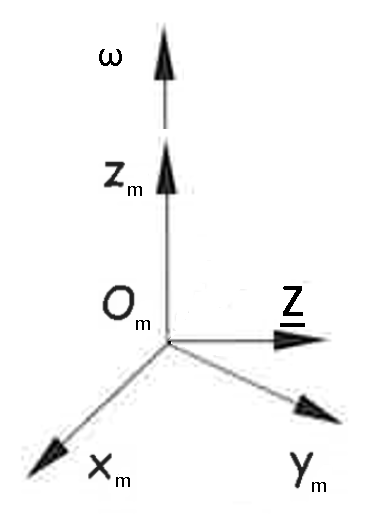
\includegraphics[width =.5\textwidth]{chapter02/immagine37}
		\end{minipage}
		\hfill
		\begin{minipage}{.5\textwidth}
		Il vettore $\underline{\omega}$ essendo parallelo all'asse $z_m$ avrà componenti solo lungo tale direzione
		\begin{equation*}
		\underline{\omega} =
			\begin{Bmatrix}
			0\\
			0\\
			\omega_z
			\end{Bmatrix}
			= 0 \cdot \mathbf{i_m} + \, 0 \cdot \mathbf{j_m} + \, \omega_z \cdot \mathbf{k_m}
		\end{equation*}
		Il vettore $\mathbf{z}$ che idenifica la posizione del punto P rispetto all'origine della terna mobile avrà coordinate rispetto alla stessa terna:
		\begin{equation*}
			\mathbf{z} = 
			\begin{Bmatrix}
				\,^mx_P \\
				\,^my_P \\
				\,^mz_P \\ 
			\end{Bmatrix}
			= \,^mx_P \cdot \mathbf{i_m} + \,^my_P \cdot \mathbf{j_m} +\,^mz_P \cdot \mathbf{k_m} 
		\end{equation*}
		\end{minipage}
		\vspace{1mm}
		
		Sotto tali ipotesi procediamo a risolvere anaiticamente ogni singolo membro del terzo termine  dell'equazione dell'accelerazione di un punto P solidale ad una terna mobile rispetto ad un osservatore assoluto.
		
		\begin{enumerate}
			\item
				 \begin{equation*}
				 	\begin{split}
				 		\underline{\omega} \wedge \mathbf{z} =	\begin{vmatrix}
				 				\mathbf{i_m} & \mathbf{j_m} & \mathbf{k_m}\vspace{1mm}\\
				 				0 & 0 & \omega_z\\
				 				x_P & y_P & z_P\\
				 			\end{vmatrix}
				 			&= - \, \omega_z \, (y_P \, \mathbf{i_m} \, - \, x_P \, \mathbf{j_m})\\
				 			&= (-\, y_P\, \omega_z ) \, \mathbf{i_m} \, + \, (x_P \, \omega_z) \, \mathbf{j_m} + 0 \, \mathbf{k_m}\\
				  	\end{split}
				  \end{equation*}
				  
				  \item
				  	\begin{equation*}
				  		\begin{split}
				  			\underline{\omega} \wedge (\underline{\omega} \wedge \mathbf{z}) =
				  				\begin{vmatrix}
				  					\mathbf{i_m} & \mathbf{j_m} & \mathbf{k_m}\vspace{1mm}\\
				  					0 & 0 & \omega_z\\
				  					x_P & y_P & z_P\\
				  				\end{vmatrix}
				  				&= -\, \omega_z \,(x_P \, \omega_z \, \mathbf{i_m} \, + \, \omega_z \, y_P \, \mathbf{j_m})\\
				  				&= (-\, \omega_z^2 \, x_P) \, \mathbf{i_m} \, + \, (-\, \omega_z^2 \, y_P) \, \mathbf{j_m} \, + \, 0\, \mathbf{k_m}\\
\\
				  				&= -\, \omega_z^2 \, \underbrace{(x_P \, \mathbf{i_m} \, +\, y_p \, \mathbf{j_m})}_{ \mathbf{\emph{r}}}
						\end{split}
				  	\end{equation*}
				  	$\mathbf{r}$ \hspace{3mm} rappresenta la proiezione di $\mathbf{z}  = \,^mx_P \cdot \mathbf{i_m} + \,^my_P \cdot \mathbf{j_m} +\,^mz_P \cdot \mathbf{k_m} $ sul piano descritto dagli assi della terna mobile ($x_m , y_m$) ed è quindi ortogonale al vettore $\omega$
		\end{enumerate}
		
		L'equazione dell'accelerazione del punto P rispetto alla terna fissa:
			\begin{equation*}
			\begin{split}
					\mathbf{a_P} &= \ddot{\underline{\rho}} + \, \dot{\underline{\omega}} \wedge \mathbf{z} + \, \underline{\omega} \wedge (\underline{\omega}\wedge \mathbf{z})\\
					&= \ddot{\underline{\rho}} + \, \dot{\underline{\omega}} \wedge \mathbf{z} - \, \omega^2 \, \mathbf{r}
			\end{split}	
			\end{equation*}
		
			dove: 
			\begin{align*}
				 \ddot{\underline{\rho}}  &=  \emph{è l'accelerazione della terna mobile}\\
				  \dot{\underline{\omega}} \wedge \mathbf{z} &= \emph{è l'accelerazione tangenziale del punto, in virtù del fatto che la sua}\\
				  & \emph{direzione è tangenziale al punto di rotazione}\\
				  - \omega^2 \, \mathbf{r} &= \emph{è l'accelerazione centripeta del punto, in virtù del fatto che il vettore risultante punta verso}\\
				  & \emph{ l'asse di rotazione}
			\end{align*}
		
		
		Non è sempre necessario, né conveniente, fissare una terna ad ogni corpo rigido del nostro sistema. Le relazioni precedenti possono essere espresse anche riferendoci alla sola terna fissa.		
		
		\begin{minipage}{.5\textwidth}
		Nota la posizione, la velocità, l'accelerazione di un punto $P_1$ appartenente al corpo rigido e il vettore velocità angolare, si possono calcolare le posizioni, le velocità e le accelerazioni di qualsiasi altro punto $P_2$ appartenente al corpo rigido:
				\begin{align*}
					\mathbf{P_2} &= \mathbf{P_1} + \mathbf{z}\\
					\dot{\mathbf{P_2}} &= \dot{\mathbf{P_1}}  + \dot{\underline{\theta}} \wedge \mathbf{z}\\
					\ddot{\mathbf{P_2}} &= \ddot{\mathbf{P_1}}  +  \ddot{\underline{\theta}} \wedge \mathbf{z} + \dot{\underline{\theta}} \wedge (\dot{\underline{\theta}} \wedge \mathbf{z})\\
				\end{align*}	
		\end{minipage}
		\hfill
		\begin{minipage}{.5\textwidth}
			\centering
			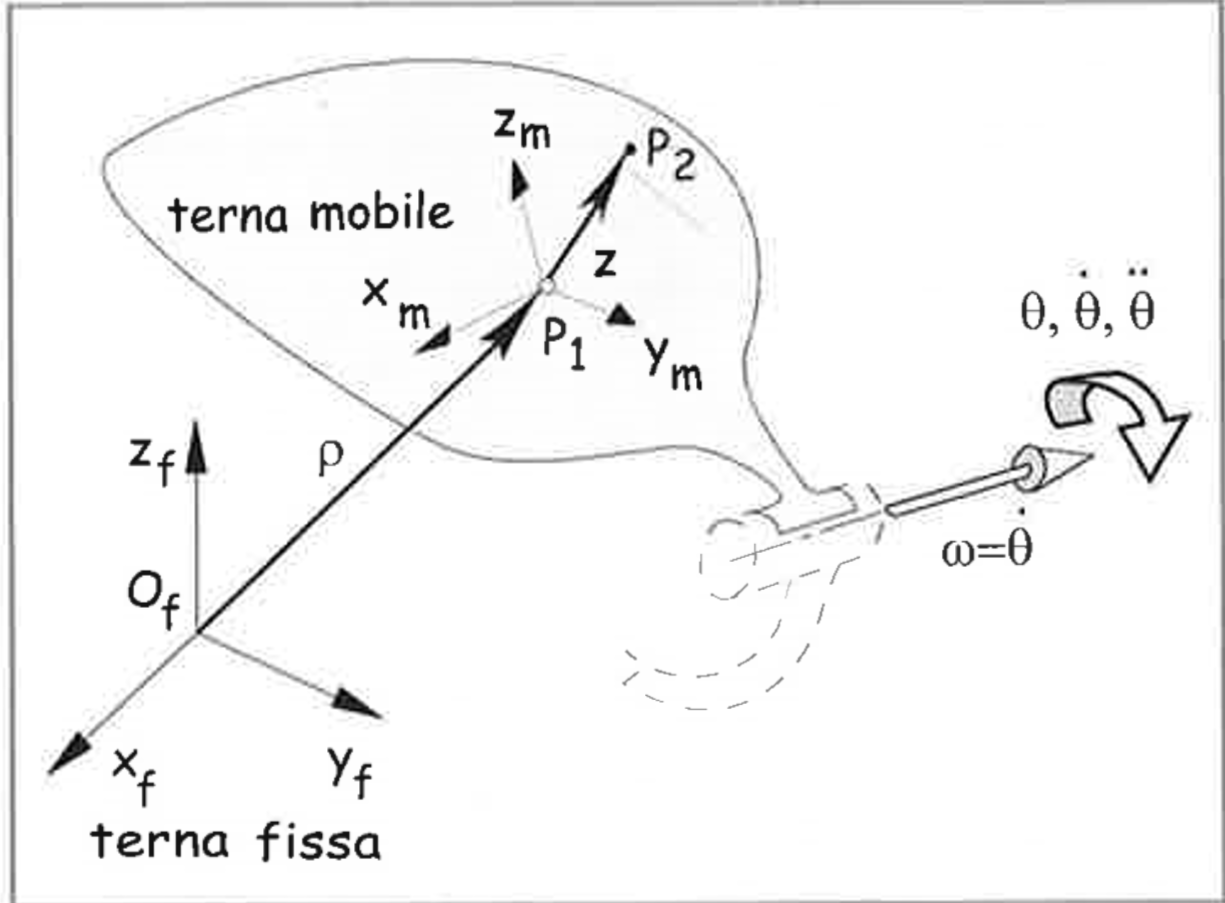
\includegraphics[width=.8\textwidth]{chapter02/immagine38}
		\end{minipage}
		
				\subsection{Cinematica di un corpo nel piano}
		
				È utile scrivere le relazioni vettoriali precedenti, valide sia nello spazio che nel piano, in forma scalare per i soli moti piani. Data la posizione, velocità e accelerazione di un punto $P_1$ di un corpo rigido, la velocità e l'accelerazione angolare di un qualsivoglia punto $P_2$ del corpo rigido sono date da:
				
		\begin{minipage}{.45\textwidth}
			\begin{align*}
			\begin{Bmatrix}
				x_2\\
				y_2
			\end{Bmatrix}
			&= 
			\begin{Bmatrix}
				x_1\\
				y_1
			\end{Bmatrix}
			+
			\begin{Bmatrix}
				a_x\\
				a_y
			\end{Bmatrix}\\
			\\
			\begin{Bmatrix}
				\dot{x_2}\\
				\dot{y_2}
			\end{Bmatrix}
			&= 
			\begin{Bmatrix}
				\dot{x_1}\\
				\dot{y_1}
			\end{Bmatrix}
			+ \, \dot{\theta}\,
			\begin{Bmatrix}
				-\, a_y\\
				a_x
			\end{Bmatrix}\\
			\\
				\begin{Bmatrix}
				\ddot{x_2}\\
				\ddot{y_2}
			\end{Bmatrix} & =
										\begin{Bmatrix}
											\ddot{x_1}\\
											\ddot{y_1}
										\end{Bmatrix}
										+ \ddot{\theta} \,
										\begin{Bmatrix}
											- \, a_y\\
											a_x
										\end{Bmatrix}
										+ \, \dot{\theta} \,
										\begin{Bmatrix}
											-\,\dot{\theta} \, a_x\\
											-\, \dot{\theta} \, a_y
										\end{Bmatrix}\vspace{2mm}\\
							&= 
									\begin{Bmatrix}
										\ddot{x_1}\\
										\ddot{y_1}
									\end{Bmatrix}
									+ \ddot{\theta} \,
									\begin{Bmatrix}
										- \, a_y\\
										a_x
									\end{Bmatrix}
									-\, \dot{\theta}^2\,
									\begin{Bmatrix}
										a_x\\
										a_y
									\end{Bmatrix}\vspace{2mm}\\
				\mathbf{a_2} &= \mathbf{a_1} \, + \, \dot{\underline{\omega}} \wedge \mathbf{z} \, -\, \omega^2 \, \mathbf{r}
		\end{align*}				
		\end{minipage}
		\hfill
		\begin{minipage}{.45\textwidth}
		\centering
			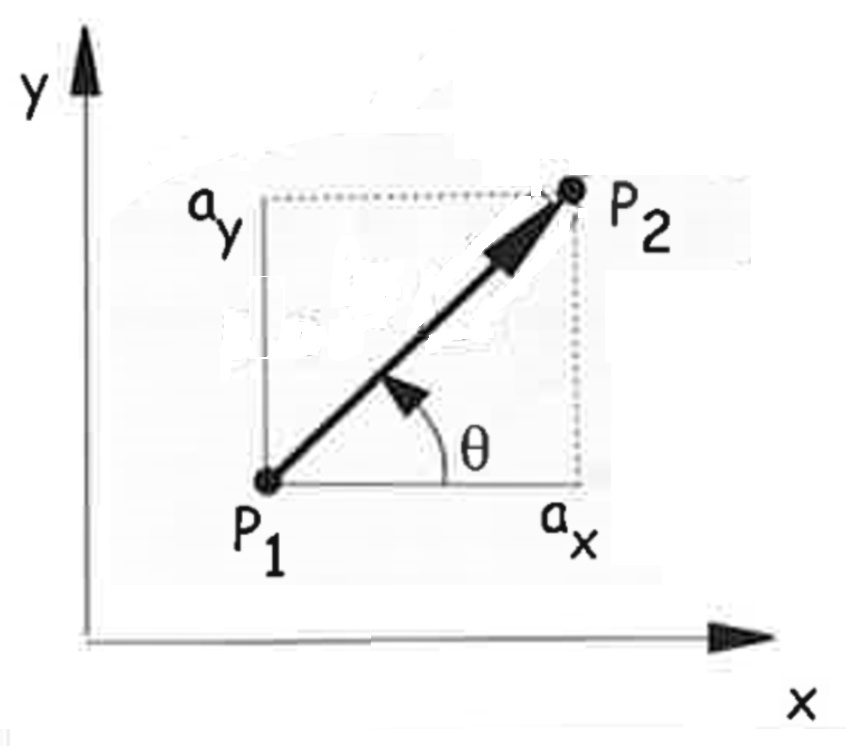
\includegraphics[width = .65\textwidth]{chapter02/immagine39}

		\begin{eqnarray*}
			a_x = a \, \cos{\theta}\quad &\quad \dot{a_x} = -\, a \, \dot{\theta} \, \sin{\theta} \,= \, - \, \dot{\theta} \, a_y\\
			a_y = a \, \sin{\theta} \quad & \quad \dot{a_y} = a \, \dot{\theta} \, \cos{\theta} \, = \, \dot{\theta} \, a_x
		\end{eqnarray*}
		\end{minipage}
	
		\vspace{2mm}
		Quest'ultima relazione è nota con il nome di \textbf{teorema di Rivals}

		\subsection{Matrice di rotazione}
			Consideriamo un sistema di riferimento ed un vettore $\mathbf{v_1}$. Vogliamo calcolare le componenti del vettore $\mathbf{v_2}$ che otteniamo ruotando $\mathbf{v_1}$ di un angolo $\theta$. Le componenti di $\mathbf{v_2}$ risultano:
			
			\vspace{2mm}
			\begin{minipage}{.5\textwidth}
				\centering
				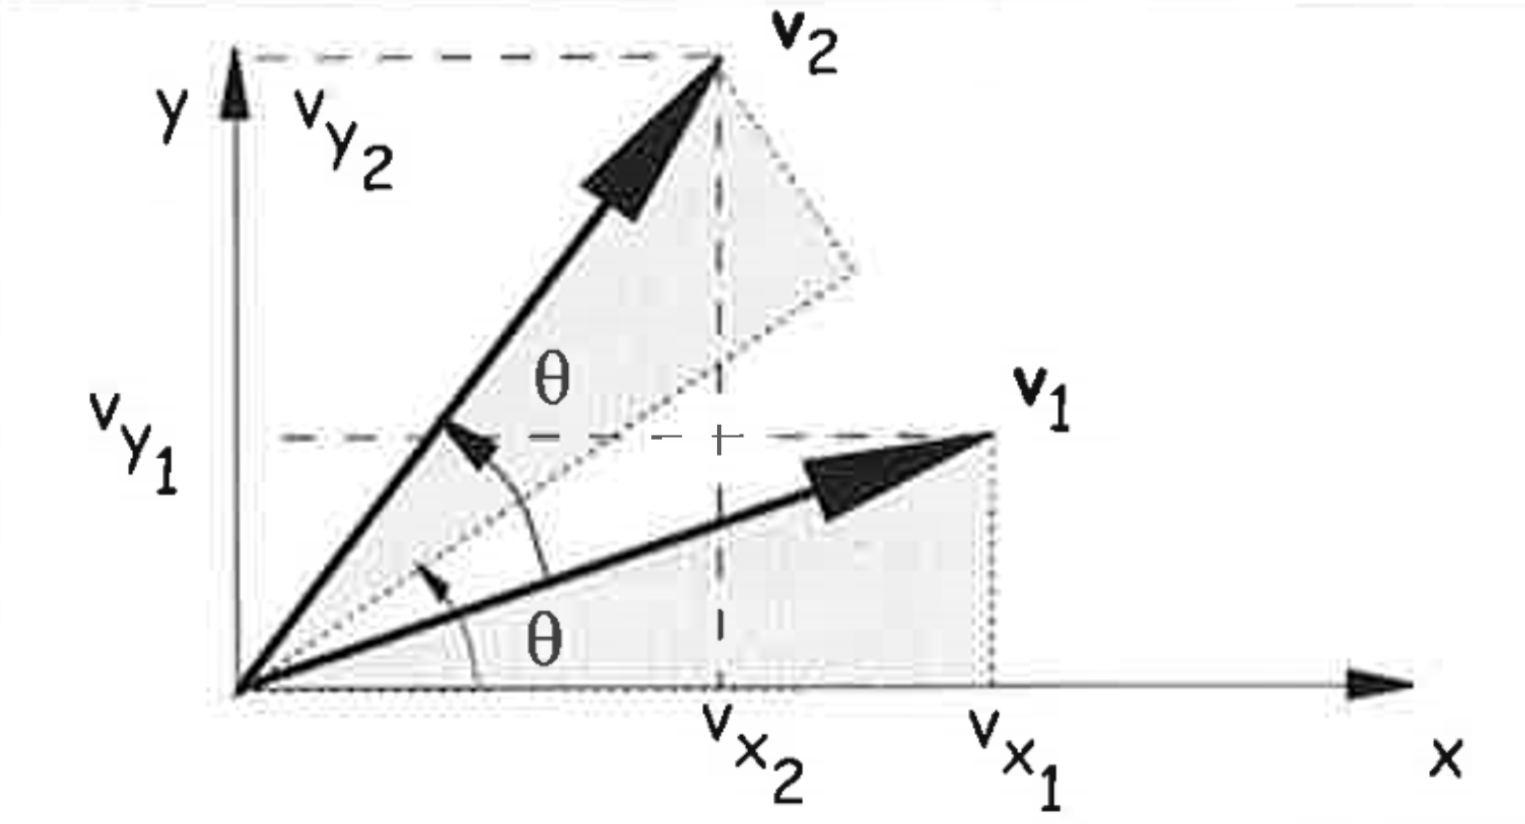
\includegraphics[width=.8\textwidth]{chapter02/immagine40}
			\end{minipage}
			\hfill
			\begin{minipage}{.5\textwidth}
				\begin{equation*}
					\begin{split}
						v_{2x} &= v_{1x} \, \cos{\theta} \,- \, v_{1y} \, \sin{\theta}\\
						v_{2y} &= v_{1x} \, \sin{\theta} \,+ \, v_{1y} \, \cos{\theta}\\
					\end{split}
				\end{equation*}
				che possono essere rappresentate in forma matriciale in funzione delle coordinate di $\mathbf{v_1}$:
				\begin{equation*}
					\begin{Bmatrix}
						v_{2x}\\
						v_{2y}
					\end{Bmatrix}
					= 
					\begin{bmatrix}
					\cos{\theta} & -\,\sin{\theta}\\
					\sin{\theta} &  \cos{\theta}
					\end{bmatrix}
					\begin{Bmatrix}
						v_{1x}\\
						v_{1y}
					\end{Bmatrix}
				\end{equation*}
			\end{minipage}

\vspace{4mm}
		La matrice che lega gli elementi del vettore $\mathbf{v_2}$ a quelle del vettore $\mathbf{v_1}$ è detta \textbf{Matrice di rotazione}. La Matrice di rotazione, dunque, è un operatore di rotazione che applicato ad un vettore qualsiasi ritorna la sua rotazione di angolo $\theta$ (che è anche l'unico parametro dell'operatore).

		\subsection{Trasformazione di coordinate}
			Un'applicazione alternativa della matrice di rotazione è la traformazione di coordinate di due sistemi di riferimento.
			Consideriamo due sistemi di riferimento aventi origine in comune, uno fisso e l'altro mobile, e che il secondo sistema sia ruotato di angolo $\theta$ rispetto al primo.\newline
			Vediamo come note le coordinate di un punto P rispetto al sistema mobile si possano calcolare le coordinate di P rispetto al sistema di riferimento fisso indicato con l'apice \emph{f}.
					
			\begin{minipage}{.5\textwidth}
			\begin{align*}
						\,^fx_P &= \, ^mx_P \, \cos{\theta} \, - \, \,^my_P \, \sin{\theta}\\
						\,^fy_P &= \, ^mx_P \, \sin{\theta} \, + \, \,^my_P \, \cos{\theta}
			\end{align*}
					Si può notare che il calcolo è analogo a quello visto per la rotazione di un vettore, in quanto possiamo immaginare l'operazione di cambio di coordinate come una rotazione del sistema di riferimento mobile a partire da una condizione iniziale coincidente con quello fisso.\newline
			\end{minipage}
			\hfill
			\begin{minipage}{.5\textwidth}
				\centering
				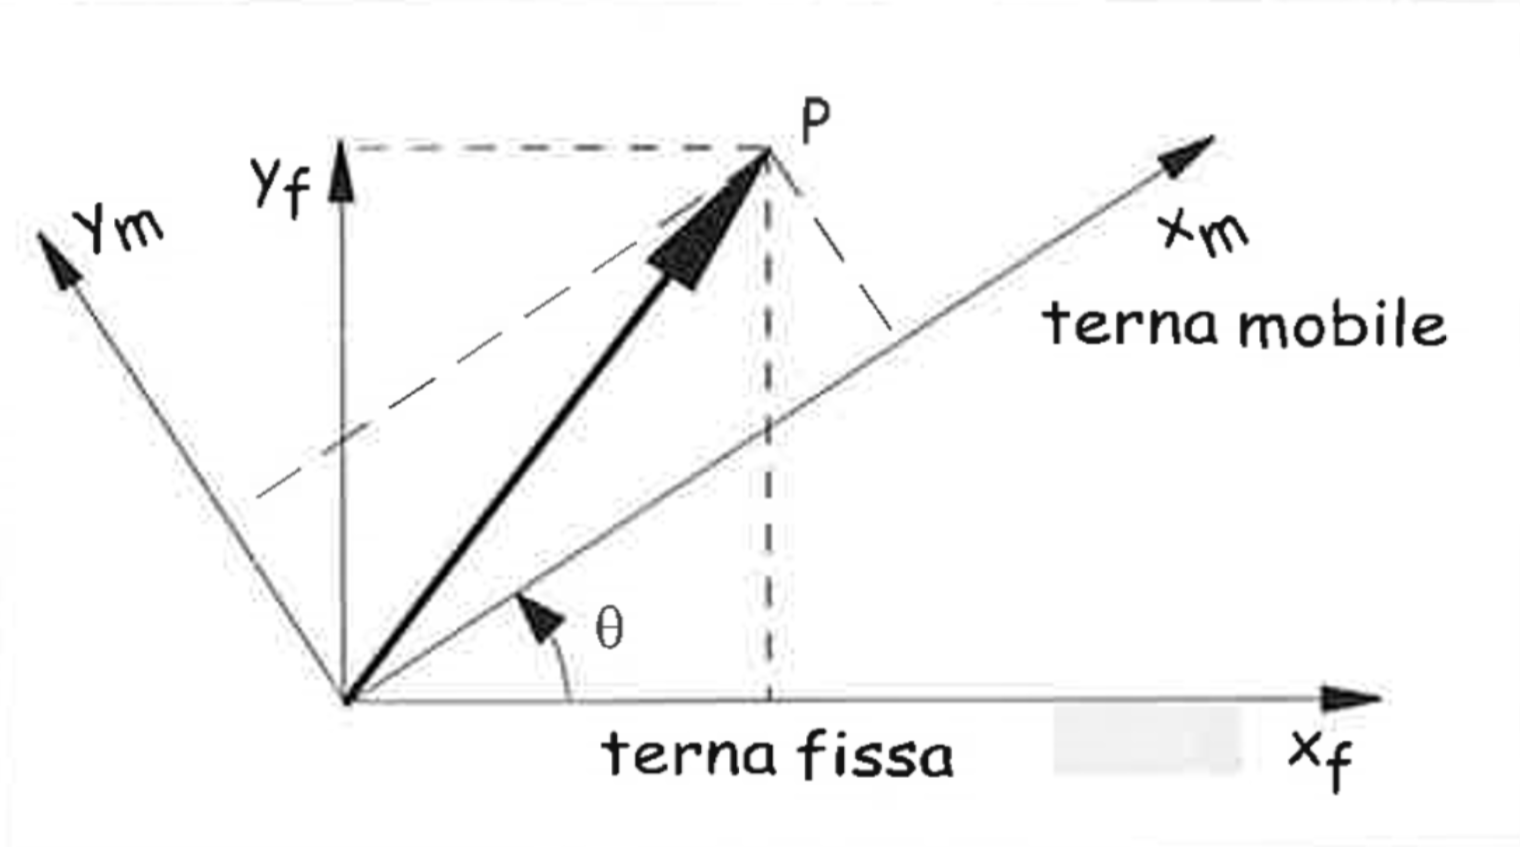
\includegraphics[width=.8\textwidth]{chapter02/immagine41}
			\end{minipage}

			La rotazione del sistema di riferimento mobile si porterà dietro tutti i vettori a lui solidale.\newline
			In forma matriciale il cambiamento di coordinate risulta essere:
		\begin{equation*}
			\leftidx{^f}{\begin{Bmatrix}
				x_P\\
				y_P
			\end{Bmatrix}}
			=
			\leftidx{_m^f}{\begin{bmatrix}
				\cos{\theta} & -\,\sin{\theta}\\
				\sin{\theta} &  \cos{\theta}
			\end{bmatrix}}\quad
			\leftidx{^m}{\begin{Bmatrix}
				x_P\\
				y_P
			\end{Bmatrix}}
		\end{equation*}
		
		La matrice di rotazione così rappresentata è rappresentativa della rotazione che da {\itshape f} (apice) va a m (pedice), assume il significato di operatore che identifica la rotazione/posizione di un sistema di riferimento ad un altro e può essere rapresentato sinteticamente dall'espressione $\,^f\{P\} = \leftidx{^f_m}{\{R\}} \,\, ^m\{P\}$.\newline
		
		Osservazioni: Le colonne della matrice di rotazione R nascondono un significato intrinseco: esse infatti coincidono con le componenti dei versori degli assi $x_m ,y_m $ rispetto a $x_f , y_f$ , cioè contiene i coseni direttori dell'asse x e y.
		Da tale proprietà si può facilmente notare che la matrice di rotazione R è ortonormale, ovvero la sua inversa coincide con la sua trasposta
		\[ \leftidx{^f_m}{\begin{bmatrix}R\end{bmatrix}}{^{-1}} \quad = \quad \leftidx{^f_m}{\begin{bmatrix}R\end{bmatrix}}{^T} \quad = \quad \leftidx{^m_f}{\begin{bmatrix}R\end{bmatrix}}\]

		Di conseguenza ponendoci solidali alla terna mobile, la matrice di rotazione da f a m può essere ottenuta ponendo le componenti dei versori della terna fissa proiettata sulla terna mobile sulle sue colonne.
			\[\leftidx{^f_m}{\begin{bmatrix}
				\, \mathbf{i_f} & \mathbf{j_f}\,
									\end{bmatrix}}
				=
				\leftidx{^f_m}{\begin{bmatrix}
					\cos{\theta} & \sin{\theta}\\
					-\,\sin{\theta} & \cos{\theta}
				\end{bmatrix}}\]

			Verifichiamo rapidamente che la matrice di rotazione è ortonormale verificando che il prodotto tra la matrice di rotazione e la sua trasposta ritorni la matrice identità. In questo modo avremo la certezza che l'inversa e la trasposta coincidano con la stessa matrice.
			\begin{proof}
				\begin{equation*}
					\begin{bmatrix}
						\cos{\theta} & \sin{\theta}\\
						-\, \sin{\theta} & \cos{\theta}
					\end{bmatrix}
					\begin{bmatrix}
						\cos{\theta} & -\, \sin{\theta}\\
						\sin{\theta} & \cos{\theta}
					\end{bmatrix}
					=
					\begin{bmatrix}
						\cos^2{\theta}\,+\,\sin^2{\theta} & -\, \sin{\theta}\,\cos{\theta} \,+\,\sin{\theta}\,\cos{\theta}\\
						-\, \sin{\theta}\,\cos{\theta} \,+\,\sin{\theta}\,\cos{\theta} & \cos^2{\theta}\,+\,\sin^2{\theta}
					\end{bmatrix}
					=
					\begin{bmatrix}
						1 & 0\\
						0 & 1
					\end{bmatrix}
				\end{equation*}\qedhere
			\end{proof}

			La matrice di traformazione ci consente di riscrivere la formula fondamentale della cinematica, nel caso in cui la posizione del punto di cui si vuole calcolare la velocità e l'accelerazione è nota rispetto ad un sistema solidale al corpo rigido.\newline
			Le equazioni che esprimono la posizione, la velocità e l'accelerazione di un generico punto P diventano:

			\begin{itemize}
				\item {\scshape{\bfseries caso 1}}: Origini coincidenti ($\underline{\rho} = 0$)
					\begin{equation*}
						\begin{split}
							\mathbf{P} &= \cancelto{_0}{\underline{\rho}} + \mathbf{z}\\
							\leftidx{^f}{\begin{Bmatrix}x \\ y\end{Bmatrix}} &= \leftidx{^f_m}{\begin{bmatrix}R\end{bmatrix}}\quad \leftidx{^m}{\begin{Bmatrix}x \\ y\end{Bmatrix}}\\
							\\
							 \leftidx{^f}{\begin{Bmatrix}\dot{x} \\ \dot{y} \end{Bmatrix}} &= \frac{d}{dt}(\begin{bmatrix}R\end{bmatrix} \quad\!\! \leftidx{^m}{\begin{Bmatrix}x \\ y\end{Bmatrix}})
						\end{split}
					\end{equation*}
					Si osserva che:
					\begin{itemize}
						\item la derivata di $ \leftidx{^m}{\begin{Bmatrix}x \\ y\end{Bmatrix}} = 0$ dato che, per ipotesi di corpo rigido, il vettore in questione risulta costante.
						\item La matrice di rotazione è funzione di un unico parametro $\theta(t)$, perciò:
						\begin{equation*}
							\frac{d}{dt}\begin{bmatrix}R\end{bmatrix} = 
								\begin{bmatrix}
									-\, \dot{\theta}\,\sin{\theta} & -\,\dot{\theta}\,\cos{\theta}\\
									\dot{\theta}\, \cos{\theta} & -\,\dot{\theta}\,\sin{\theta}
								\end{bmatrix} = 
								\dot{\theta}\,\begin{bmatrix}
									-\,\sin{\theta} & -\,\cos{\theta}\\
									\cos{\theta} & -\,\sin{\theta}
								\end{bmatrix}
						\end{equation*}
						L'equazione così ottenuta può essere riscritta in funzione della matrice di rotazione R introducendo una matrice di permutazione P:
						\begin{equation*}
							\frac{d}{dt} \begin{bmatrix}R\end{bmatrix} = \dot{\theta}\,\begin{bmatrix}
									-\,\sin{\theta} & -\,\cos{\theta}\\
									\cos{\theta} & -\,\sin{\theta}
								\end{bmatrix}
								= \dot{\theta}\,\begin{bmatrix}
										\cos{\theta} & -\,\sin{\theta}\\
										\sin{\theta} &  \cos{\theta}
								\end{bmatrix}
								\begin{bmatrix}
									0 & -1\\
									1 & 0
								\end{bmatrix}
								=  \dot{\theta}\,\begin{bmatrix}R\end{bmatrix}\, \begin{bmatrix}P\end{bmatrix}
						\end{equation*}
					\end{itemize}
					Di conseguenza:
					\begin{equation*}
						\begin{split}
							 \leftidx{^f}{\begin{Bmatrix}\dot{x} \\ \dot{y} \end{Bmatrix}} &= \frac{d}{dt}(\begin{bmatrix}R\end{bmatrix}) \quad\!\! \leftidx{^m}{\begin{Bmatrix}x \\ y\end{Bmatrix}}\\
							 &=  \dot{\theta}\,\begin{bmatrix}R\end{bmatrix}\, \begin{bmatrix}P\end{bmatrix}  \leftidx{^m}{\begin{Bmatrix}x \\ y\end{Bmatrix}}\\
							 &=   \dot{\theta}\,\begin{bmatrix}R\end{bmatrix}\,
							 \begin{bmatrix}
									0 & -1\\
									1 & 0
								\end{bmatrix}\,
								 \leftidx{^m}{\begin{Bmatrix}x \\ y\end{Bmatrix}}\\
							&= \dot{\theta}\,\begin{bmatrix}R\end{bmatrix}\,  \leftidx{^m}{\begin{Bmatrix}-\,y \\ x\end{Bmatrix}}
							\\
							\\
							 \leftidx{^f}{\begin{Bmatrix}\ddot{x} \\ \ddot{y} \end{Bmatrix}} &= \frac{d}{dt}( \dot{\theta}\,\begin{bmatrix}R\end{bmatrix}\, \begin{bmatrix}P\end{bmatrix}\leftidx{^m}{\begin{Bmatrix}x \\ y\end{Bmatrix}})\\
							&= \frac{d}{dt}( \dot{\theta}\,\begin{bmatrix}R\end{bmatrix}\, \begin{bmatrix}P\end{bmatrix})\leftidx{^m}{\begin{Bmatrix}x \\ y\end{Bmatrix}}\\
							&= \ddot{\theta}\,\begin{bmatrix}R\end{bmatrix}\, \begin{bmatrix}P\end{bmatrix}
							\leftidx{^m}{\begin{Bmatrix}x \\ y\end{Bmatrix}}
							\,+\,\dot{\theta}^2\,\begin{bmatrix}R\end{bmatrix}\, \begin{bmatrix}P\end{bmatrix}\,\begin{bmatrix}P\end{bmatrix}\,
							\leftidx{^m}{\begin{Bmatrix}x \\ y\end{Bmatrix}}\\
							&= \ddot{\theta}\,\begin{bmatrix}R\end{bmatrix}\, \begin{bmatrix}P\end{bmatrix}
							\leftidx{^m}{\begin{Bmatrix}x \\ y\end{Bmatrix}}
							\,+\,\dot{\theta}^2\,\begin{bmatrix}R\end{bmatrix}\,  \begin{bmatrix}
									0 & -1\\
									1 & 0
								\end{bmatrix}\,
								 \begin{bmatrix}
									0 & -1\\
									1 & 0
								\end{bmatrix}\,
							\leftidx{^m}{\begin{Bmatrix}x \\ y\end{Bmatrix}}\\
							& =  \ddot{\theta}\,\begin{bmatrix}R\end{bmatrix}\, \begin{bmatrix}P\end{bmatrix}
							\leftidx{^m}{\begin{Bmatrix}x \\ y\end{Bmatrix}}
							\,+\,\dot{\theta}^2\,\begin{bmatrix}R\end{bmatrix}\,  \begin{bmatrix}
									-1 & 0\\
									0 & -1
								\end{bmatrix}\,
							\leftidx{^m}{\begin{Bmatrix}x \\ y\end{Bmatrix}}\\
							&=  \ddot{\theta}\,\begin{bmatrix}R\end{bmatrix}\, \begin{bmatrix}P\end{bmatrix}
							\leftidx{^m}{\begin{Bmatrix}x \\ y\end{Bmatrix}}
							\,-\,\dot{\theta}^2\,\begin{bmatrix}R\end{bmatrix}\,
							\leftidx{^m}{\begin{Bmatrix}x \\ y\end{Bmatrix}}\\
						\end{split}
					\end{equation*}
				\item 	 {\scshape{\bfseries caso 2}}: Origini non coincidenti ($\underline{\rho} \ne 0$)		
				
				\begin{minipage}{.5\textwidth}
					\begin{equation*}
						\begin{split}
							\,^fx_P &= \,^mx_P \, \cos{\theta}\, -\, ^my_P\,\sin{\theta}\,+\,^fx_{Om}\\
							\,^fy_P &= \,^mx_P \, \sin{\theta}\, +\, ^my_P\,\cos{\theta}\,+\,^fy_{Om}\\
							\leftidx{^f}{\begin{Bmatrix}x \\ y\end{Bmatrix}} &= 
							\leftidx{^f_m}{\begin{bmatrix}R\end{bmatrix}}\,
							\leftidx{^m}{\begin{Bmatrix}x \\ y\end{Bmatrix}}\,+\,
							\leftidx{^f}{\begin{Bmatrix}x_{Om} \\ y_{Om}\end{Bmatrix}}
						\end{split}
					\end{equation*}
				\end{minipage}
				\hfill
				\begin{minipage}{.5\textwidth}
					\centering
					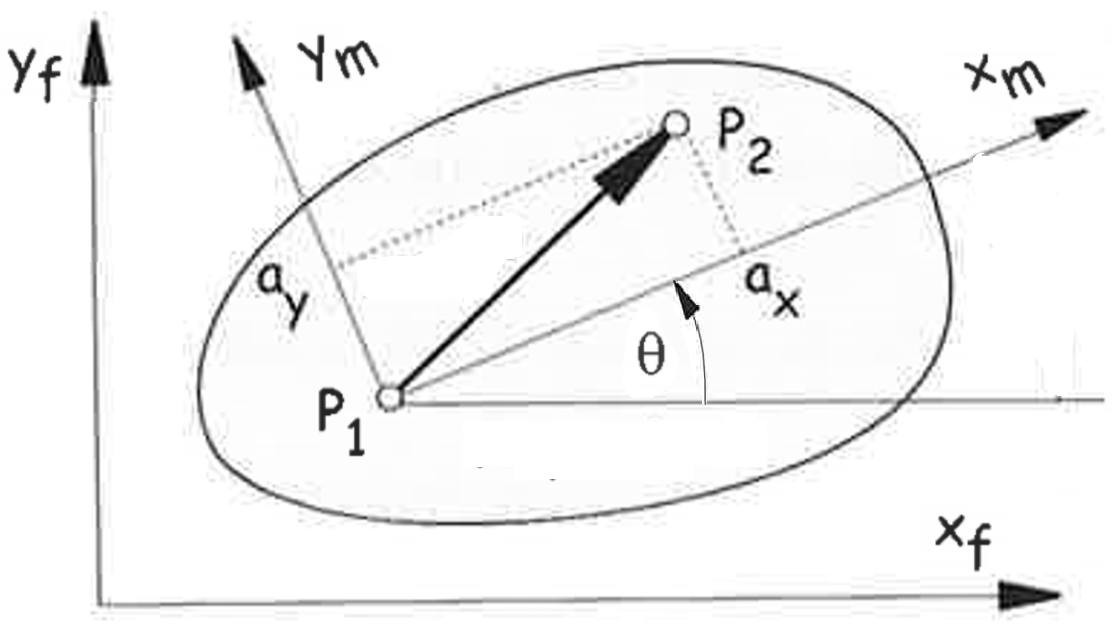
\includegraphics[width=.65\textwidth]{chapter02/immagine42}
				\end{minipage}
			\end{itemize}
	
		\subsection{Cinematica dei moti relativi}
			L'accelerazione di Coriolis fa parte della cinematica dei moti relativi: in tali condizioni il punto P non è solidale alla terna mobile, ovvero cade l'ipotesi per cui le coordinate del punto P rispetto alla terna mobile siano costanti.$ ( \mathbf{z}=(\,^mx_P(t) ,\,^my_P(t),\,^mz_P(t)))$
			
			Sia:\begin{align*}
			 \mathbf{P} &: \emph{Le coordinate del punto P in questione rispetto alla terna fissa}\\
			 \und{\rho} = \mathbf{O_fO_m} &: \emph{La distanza delle origine dei due sistemi di riferimento (mobile e fisso)}\\
			 \mathbf{z} = \mathbf{O_mP} &: \emph{Le coordinate in funzione del tempo del punto P rispetto alla terna mobile}
			\end{align*}

			\begin{equation*}
				\begin{split}
					\mathbf{P} &= \underline{\rho}\,+\,\mathbf{z}\\
					&= \underline{\rho}\, + \, ^mx_P\,\mathbf{i_m}\,+\, ^my_P\,\mathbf{j_m}\,+\, ^mz_P\,\mathbf{k_m}\\
					\\
					\frac{d}{dt}\mathbf{P} &= \dot{\underline{\rho}} \, +\, \underline{\omega}\wedge\mathbf{z}\, +\,\frac{d}{dt}\mathbf{z}
				\end{split}
			\end{equation*}
			
			Procediamo a sviluppare separatamente il termine  $\frac{d}{dt}\mathbf{z}$:
			\[
				\begin{split}
					\frac{d}{dt}\mathbf{z} &=   \, ^m\dot{x_P}\,\mathbf{i_m}\,+\, ^m\dot{y_P}\,\mathbf{j_m}\,+\, ^m\dot{z_P}\,\mathbf{k_m}\\
													&\, +\, ^mx_P\,(\underline{\omega}\wedge\mathbf{i_m})\,+\, ^my_P\,(\underline{\omega}\wedge\mathbf{j_m})\,+\, ^mz_P\,(\underline{\omega}\wedge\mathbf{k_m})\\
													\\
													&= ( \, ^m\dot{x_P}\,\mathbf{i_m}\,+\, ^m\dot{y_P}\,\mathbf{j_m}\,+\, ^m\dot{z_P}\,\mathbf{k_m})\,+\,(\underline{\omega}\wedge\mathbf{z})
				\end{split}
			\]
			
			L'equazione dell velocità del punto P rispetto alla terna fissa risulta, di conseguenza, essere:
			\[
				\frac{d}{dt}\mathbf{P} = \dot{\underline{\rho}} + \underline{\omega}\wedge\mathbf{z} + \dot{\mathbf{z}}
			\]
			dove: 
			\begin{align*}
				( \dot{\underline{\rho}} + \underline{\omega}\wedge\mathbf{z}) &: \emph{velocità di trascinamento che P avrebbe se fosse dolidale alla terna mobile}\\
				( \dot{\mathbf{z}})&: \emph{velocità relativa del punto rispetto alla terna mobile}
			\end{align*}
			\[
			\begin{split}
				\frac{d^2}{dt^2}\mathbf{P} &= \ddot{\underline{\rho}} \, +\, \dot{\underline{\omega}} \wedge\mathbf{z} \,+\, \underline{\omega}\wedge(\underline{\omega}\wedge\mathbf{z}\,+\,\dot{\mathbf{z}})\, +\, \underline{\omega}\wedge\dot{\mathbf{z}}\, +\,\ddot{\mathbf{z}}\\
				&= \ddot{\underline{\rho}}\,+\,\dot{\underline{\omega}}\wedge\mathbf{z}\,+\, \underline{\omega}\wedge(\underline{\omega}\wedge\mathbf{z}) \,+\,2\,\underline{\omega}\wedge\dot{\mathbf{z}} \,+\, \ddot{\mathbf{z}} 
			\end{split}
			\]
			dove:
			\begin{align*}
				 \ddot{\underline{\rho}}\,+\,\dot{\underline{\omega}}\wedge\mathbf{z}\,+\, \underline{\omega}\wedge(\underline{\omega}\wedge\mathbf{z}) &: \emph{accelerazione della terna o accelerazione di trascinamento}\\
				2\,\underline{\omega}\wedge\dot{\mathbf{z}}&: \emph{accelerazione di Coriolis}\\
				\ddot{\mathbf{z}}  &: \emph{accelerazione relativa}
			\end{align*}
			
			\subsection{Cinematica dei moti relativi nel piano}
		
		Nel caso piano le relazioni cinematiche dei moti relativi, scritte in forma scalare diventano:
		
		\begin{minipage}{.4\textwidth}
			\centering
			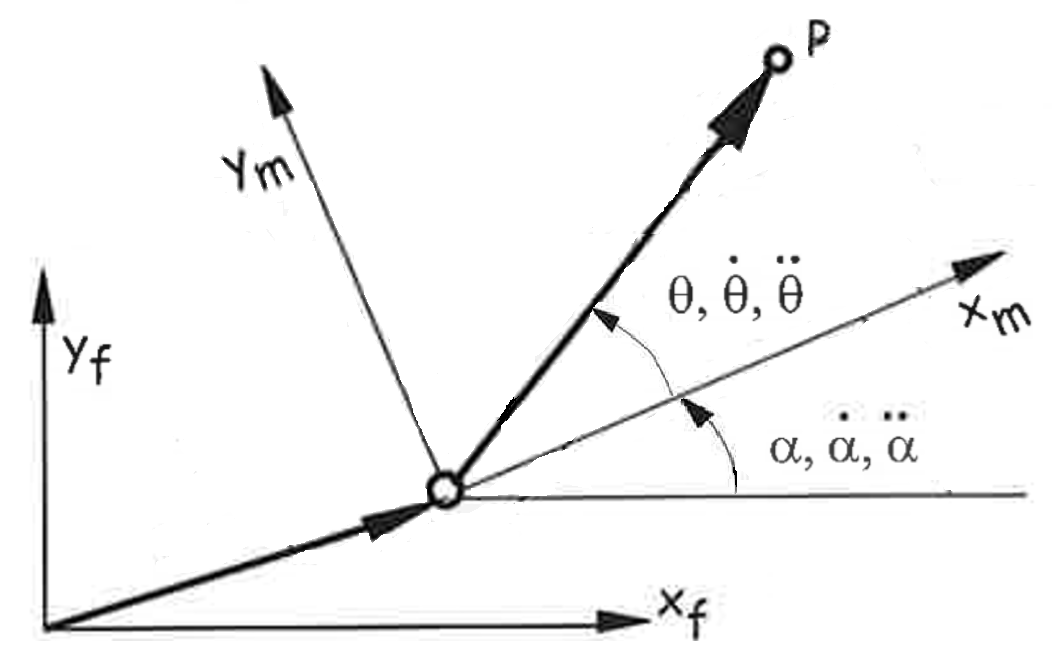
\includegraphics[width=.8\textwidth]{chapter02/immagine43}
		\end{minipage}
		\hfill
		\begin{minipage}{.6\textwidth}
			\begin{enumerate}[$\rightarrow$]
				\item \textbf{ Posizione}. Le coordinate del punto P risultano:
					\begin{equation*}
						\leftidx{^f}{\begin{Bmatrix}x_P\\y_P \end{Bmatrix}} =
						\leftidx{^f}{\begin{Bmatrix}x_{Om}\\y_{O_m} \end{Bmatrix}}\,+\,
						\leftidx{^f_m}{\begin{bmatrix}R\end{bmatrix}}\,
						\leftidx{^m}{\begin{Bmatrix} a_x \\a_y\end{Bmatrix}}
					\end{equation*}
					R indica la matrice di trasformazione che consente il passaggio dalla terna mobile \emph{m} alla terna fissa \emph{f}.
					
				\item \textbf{Velocità}. Le componenti della velocità del punto P risultano:
					\begin{equation*}
						\leftidx{^f}{\begin{Bmatrix}\dot{x_P}\\\dot{y_P} \end{Bmatrix}} =
						\leftidx{^f}{\begin{Bmatrix}\dot{x_{Om}}\\\dot{y_{O_m}} \end{Bmatrix}}\,+\,
						\leftidx{^f_m}{\begin{bmatrix}R\end{bmatrix}}\,
						\leftidx{^m}{\begin{Bmatrix}\dot{\alpha}\,
						\begin{Bmatrix}-\, a_y \\a_x\end{Bmatrix}+
						\begin{Bmatrix}\dot{a_x}\\\dot{a_y}\end{Bmatrix}
						\end{Bmatrix}}
					\end{equation*}
				\end{enumerate}
			\end{minipage}
		
			\begin{enumerate}[$\rightarrow$]
				\item \textbf{Accelerazione}. Le componenti dell'accelerazione del punto P risultano:

					\begin{equation*}
						\leftidx{^f}{\begin{Bmatrix}\ddot{x_P}\\\ddot{y_P}\end{Bmatrix}} =
						\leftidx{^f}{\begin{Bmatrix}\ddot{x_{Om}}\\\ddot{y_{Om}}\end{Bmatrix}} \, +\,
						\leftidx{^f_m}{\begin{bmatrix}R\end{bmatrix}}\,
						\leftidx{^m}{\begin{Bmatrix}\ddot{\alpha}\,
						\begin{Bmatrix}-\,a_y\\a_x\end{Bmatrix}\,
						-\dot{\alpha}^2 \, \begin{Bmatrix}a_x\\a_y\end{Bmatrix} \, +\,
						\begin{Bmatrix}\ddot{a_x}\\\ddot{a_y}\end{Bmatrix}\, +\,
						2\dot{\alpha}\,\begin{Bmatrix}-\dot{a_y}\\\dot{a_x}\end{Bmatrix}\end{Bmatrix}}
					\end{equation*}
			\end{enumerate}
		
		Precisazione: 
		\begin{itemize}
			\item nel caso spaziale il prodotto esterno in forma scalare diventa:
				\begin{align*}
					\mathbf{a}\wedge\mathbf{b} = 
					\begin{vmatrix}
						i & j & k\\
						a_x & a_y & a_z\\
						b_x & b_y & b_z
					\end{vmatrix}
					&=
					(a_y \, b_z \,-\,a_z \, b_y)\,\mathbf{i}\, +\, (a_z \, b_x \,-\,a_x \, b_z)\,\mathbf{j}\,+	\,(a_x \, b_y \,-\,a_y \, b_x)\,\mathbf{k}\\
					&=	\begin{Bmatrix}
						a_y \, b_z \,-\,a_z \, b_y\\
						a_z \, b_x \,-\,a_x \, b_z\\
						a_x \, b_y \,-\,a_y \, b_x
					\end{Bmatrix}	
					=
					\begin{bmatrix}
					0 & -a_z & a_y\\
					a_z & 0 & -a_x\\
					-a_y & a_x & 0
					\end{bmatrix}
					\begin{Bmatrix}
					b_x\\
					b_y\\
					b_z
					\end{Bmatrix}				
				\end{align*}
				
			\item nel caso piano (a perpendicolare al piano):
				\begin{align*}
					\mathbf{a}\wedge\mathbf{b} = 
					\begin{vmatrix}
						i & j & k\\
						0 & 0 & a_z\\
						b_x & b_y & b_z
					\end{vmatrix}
					&=
					(-a_z\,b_y)\mathbf{i}\, +\, (-a_z \, b_x)\,\mathbf{j}\,+ \,0\,\mathbf{k}\\
					=	\begin{Bmatrix}
						-a_z\,b_y \\
						a_z \, b_x\\
						0
					\end{Bmatrix}	
					&=
					\begin{bmatrix}
						0 & -a_z & 0\\
						a_z & 0 & 0\\
						0 & 0 & 0
					\end{bmatrix}
					\begin{Bmatrix}
					b_x\\
					b_y\\
					b_z
					\end{Bmatrix}
					=
					a_z\,
					\begin{Bmatrix}
						-b_y\\
						b_x\\
						0
					\end{Bmatrix}
				\end{align*}
		\end{itemize}